\documentclass[12pt]{article}
\pdfsuppresswarningpagegroup=1


% === Packages ===
\usepackage{amsmath, amssymb, graphicx, geometry, float}
\usepackage[colorlinks=true, linkcolor=blue]{hyperref}
\usepackage{qrcode}
\usepackage{tocloft}
\setlength{\cftbeforesecskip}{6pt}
\setlength{\cftbeforesubsecskip}{2pt}

\geometry{margin=1in}

% === Title ===
\title{Entropy Collapse: A Unified Framework Linking Entropy, Gravity, and Fundamental Particle Formation}
\author{Ismail Chajar}
\date{\today}

\begin{document}

\maketitle

\begin{abstract}
We present a unified framework proposing that entropy is the fundamental boundary condition underlying the structure of physical reality. Under extreme gravitational compression—such as inside black holes—entropy collapses from a 3D volumetric distribution to a 2D surface-projected state. This transformation governs the stabilization of mass-energy and the emergence of fundamental particles. A key element of the model is the Bruno Constant: a proportional threshold defining the collapse boundary. Supported by simulations, figure mappings, and entropy-density projections, this framework suggests that gravitational compression flattens quantum degrees of freedom, producing structured information in a lower-dimensional field.
\end{abstract}

\clearpage
\tableofcontents
\clearpage

\section{Introduction}
The Entropy Collapse Hypothesis proposes that entropy is not merely a measure of disorder, but the structural boundary condition guiding the emergence of energy, particles, and even time itself. This framework suggests that at extreme gravitational compression—such as within black holes—entropy collapses from a 3D volumetric state to a 2D surface configuration. This dimensional transition stabilizes mass-energy, leading to the formation of fundamental particles through constrained quantum behavior.

The project emerged through iterative simulation, theoretical modeling, and visual analysis, with each output timestamped and mapped to its generating script. Central to this framework is the Bruno Constant, a proportional threshold that defines the collapse boundary between volume-based entropy and its 2D surface-projected equivalent. By analyzing entropy flow, gravitational gradients, and quantum stabilization behavior, this work aims to unify Thermodynamics, General Relativity, and Quantum Mechanics under a single entropic architecture.


\section{Foundational Assumptions}
\[
S \propto k \cdot \ln(\Omega)
\]

\begin{figure}[H]
    \centering
    \includegraphics[width=0.8\textwidth]{fig_01_entropy_decay.png}
    \caption{Entropy Decay Model — Energy and Information Degradation in a High-Entropy System.}
    \label{fig:entropy_decay}
\end{figure}

\begin{itemize}
    \item Entropy is the primary organizing principle of the universe.
    \item Black holes reach a state of zero entropy at the core (0K-like stabilization).
    \item The Bruno Constant defines the collapse boundary between volumetric and surface entropy distribution.
    \item Dimensional flattening (3D → 2D) is a real physical transformation during gravitational compression.
\end{itemize}

\section{Entropy Collapse Mechanism}
\[ S = \frac{k c^3 A}{4 G \hbar} \]

\begin{figure}[H]
    \centering
    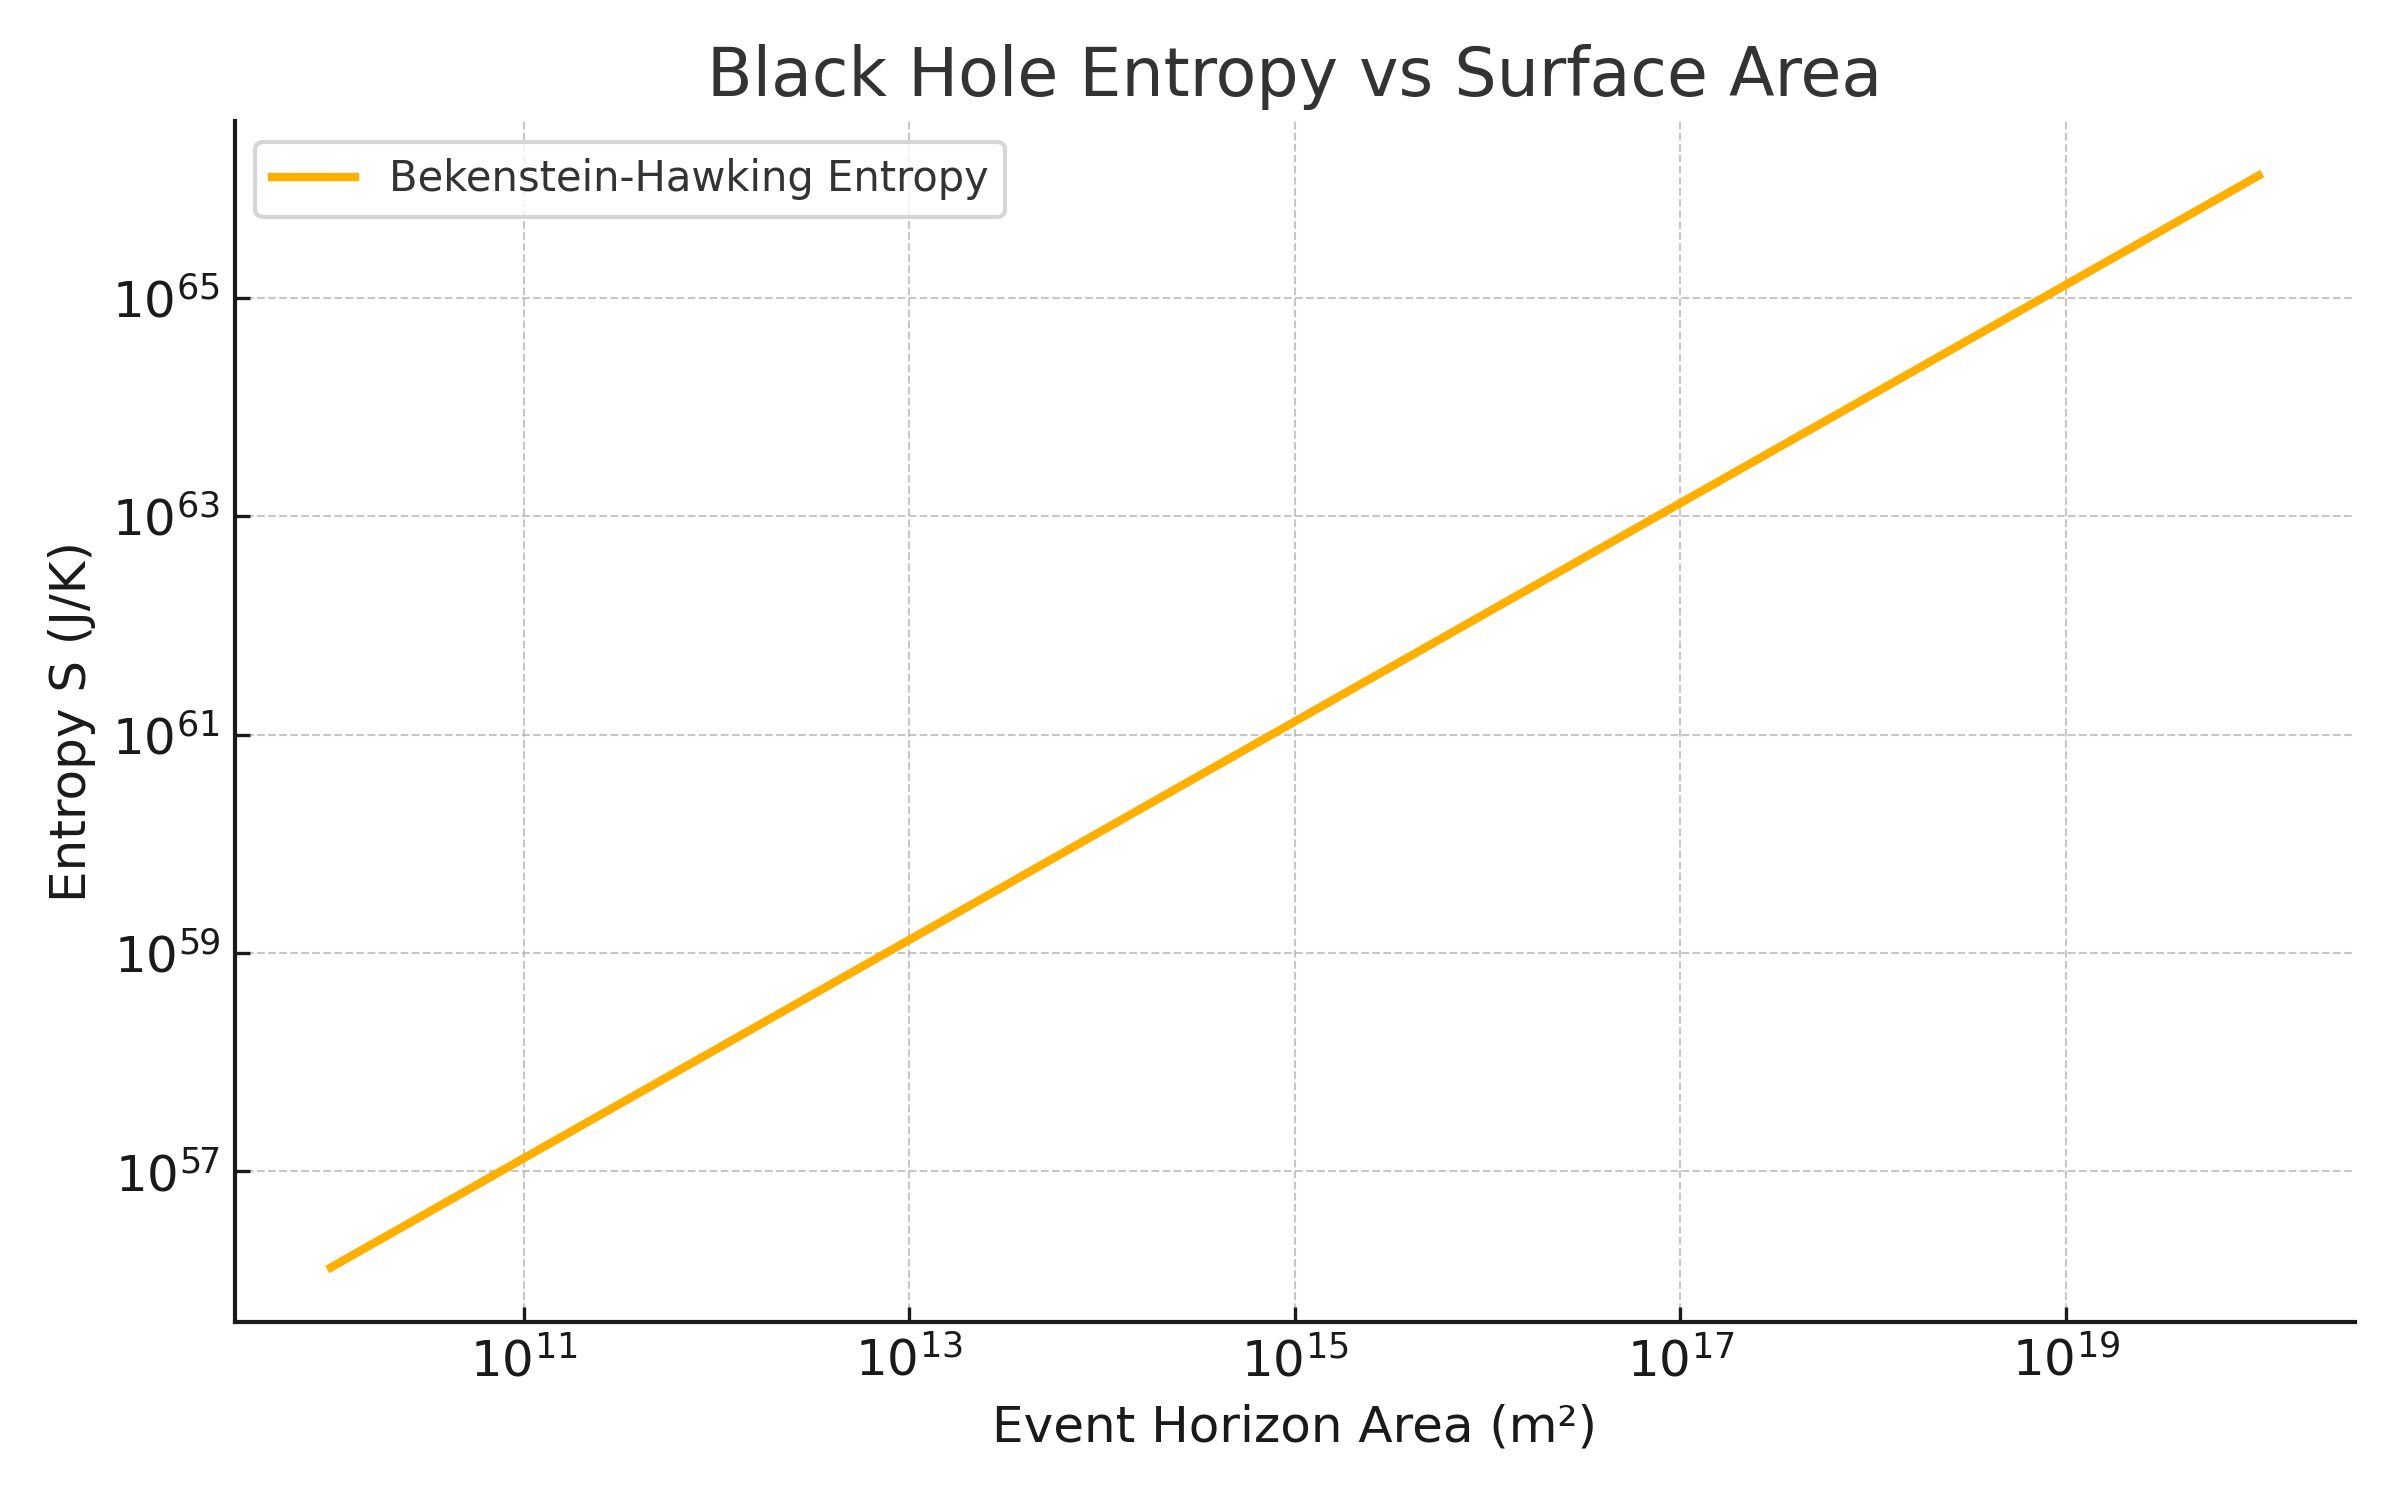
\includegraphics[width=0.8\textwidth]{fig_02_bh_entropy_area.png}
    \caption{Bekenstein-Hawking Entropy as a Function of Event Horizon Area.}
    \label{fig:bh_entropy_area}
\end{figure}

\clearpage
\section{Field Theory Formulation of Entropy Collapse}

To unify entropy, gravity, and collapse into a dynamical framework, we define entropy as a scalar field $S(x^\mu)$ over spacetime. This field is not a passive thermodynamic measure, but an active agent that interacts with spacetime geometry. 

\subsection*{Entropy as a Scalar Field}
We model entropy as a differentiable scalar field whose spatial gradient governs the emergence of gravitational effects:
\[
g(x) \propto -\nabla S(x)
\]
This gradient-based gravitational behavior aligns with the toy model (see Figure~\ref{fig_06_toy_model_entropy}).

\subsection*{Lagrangian Construction}
The field dynamics of $S$ are governed by the Lagrangian density:
\[
\mathcal{L}(S, \partial_\mu S) = \frac{1}{2} \partial_\mu S \, \partial^\mu S - \frac{\lambda}{4}(S^2 - S_c^2)^2
\]
where:
\begin{itemize}
\item $S_c$ is the collapse threshold entropy density, linked to the Bruno Constant.
\item $\lambda$ is a self-coupling term controlling collapse sharpness.
\end{itemize}

\subsection*{Field Equation and Interpretation}
Applying the Euler-Lagrange equation yields:
\[
\Box S + \lambda S(S^2 - S_c^2) = 0
\]
which shows how the field stabilizes in a low-entropy, surface-bound configuration beyond $S_c$. This offers a continuous transition from Newtonian-like behavior to holographic boundary projection.

\subsection*{Interpretation of the Bruno Constant}
The Bruno Constant $k_B$ modulates $S_c$ as a proportional cutoff:
\[
S_c = k_B \cdot S_{\text{Planck}}
\]
and serves as the thermodynamic threshold at which volumetric entropy collapses into a 2D surface structure.

As gravitational compression intensifies, matter-energy is forced into lower-entropy configurations. This behavior defines the entropy collapse mechanism. The Bruno Constant, derived through simulation and dimensional analysis, marks a specific threshold: when a system's 3D entropy volume becomes equivalent to its projected 2D entropy surface. At this collapse point, the system can no longer maintain volumetric stability, triggering a field projection onto a lower-dimensional surface.

\subsection{Equation Set and Collapse Threshold}
The following table highlights key equations central to modeling entropy collapse. Each is traceable to its simulation script and visual output, forming a cohesive chain from theoretical expression to graphical validation.

% ===============================
% Equation-to-Figure Mapping Table
% ===============================

\begin{table}[H]
\centering
\begin{tabular}{|c|l|l|l|}
\hline
\textbf{ID} & \textbf{Equation} & \textbf{Script Source} & \textbf{Linked Figure} \\
\hline
E01 & \( S = \frac{k_B c^3 A}{4 G \hbar} \) & \texttt{entropy\_BH\_base.py} & Figure~\ref{fig_02_bh_entropy_area} \\
E02 & \( \nabla \cdot \vec{g} = -\frac{\partial S}{\partial V} \) & \texttt{entropy\_gradient\_model.py} & Figure~\ref{fig_03_gradient_model} \\
E03 & \( \frac{S_{3D}}{S_{2D}} = \mathcal{B} \) & \texttt{entropy\_collapse\_threshold.py} & Figure~\ref{fig_04_collapse_threshold} \\
E04 & \( \vec{\Psi}(x, t) \propto \delta(S) \cdot e^{-iEt/\hbar} \) & \texttt{entropy\_quantum\_test.py} & Figure~\ref{fig_05_wavefunction_stability} \\
\hline
\end{tabular}
\caption{Core equations used in modeling entropy collapse and Bruno Constant threshold.}
\label{tab:equation-map}
\end{table}

\clearpage

% ===============================
% Figures Linked to Table Entries
% ===============================

% --- Figure for E01 ---
\begin{figure}[H]
\centering
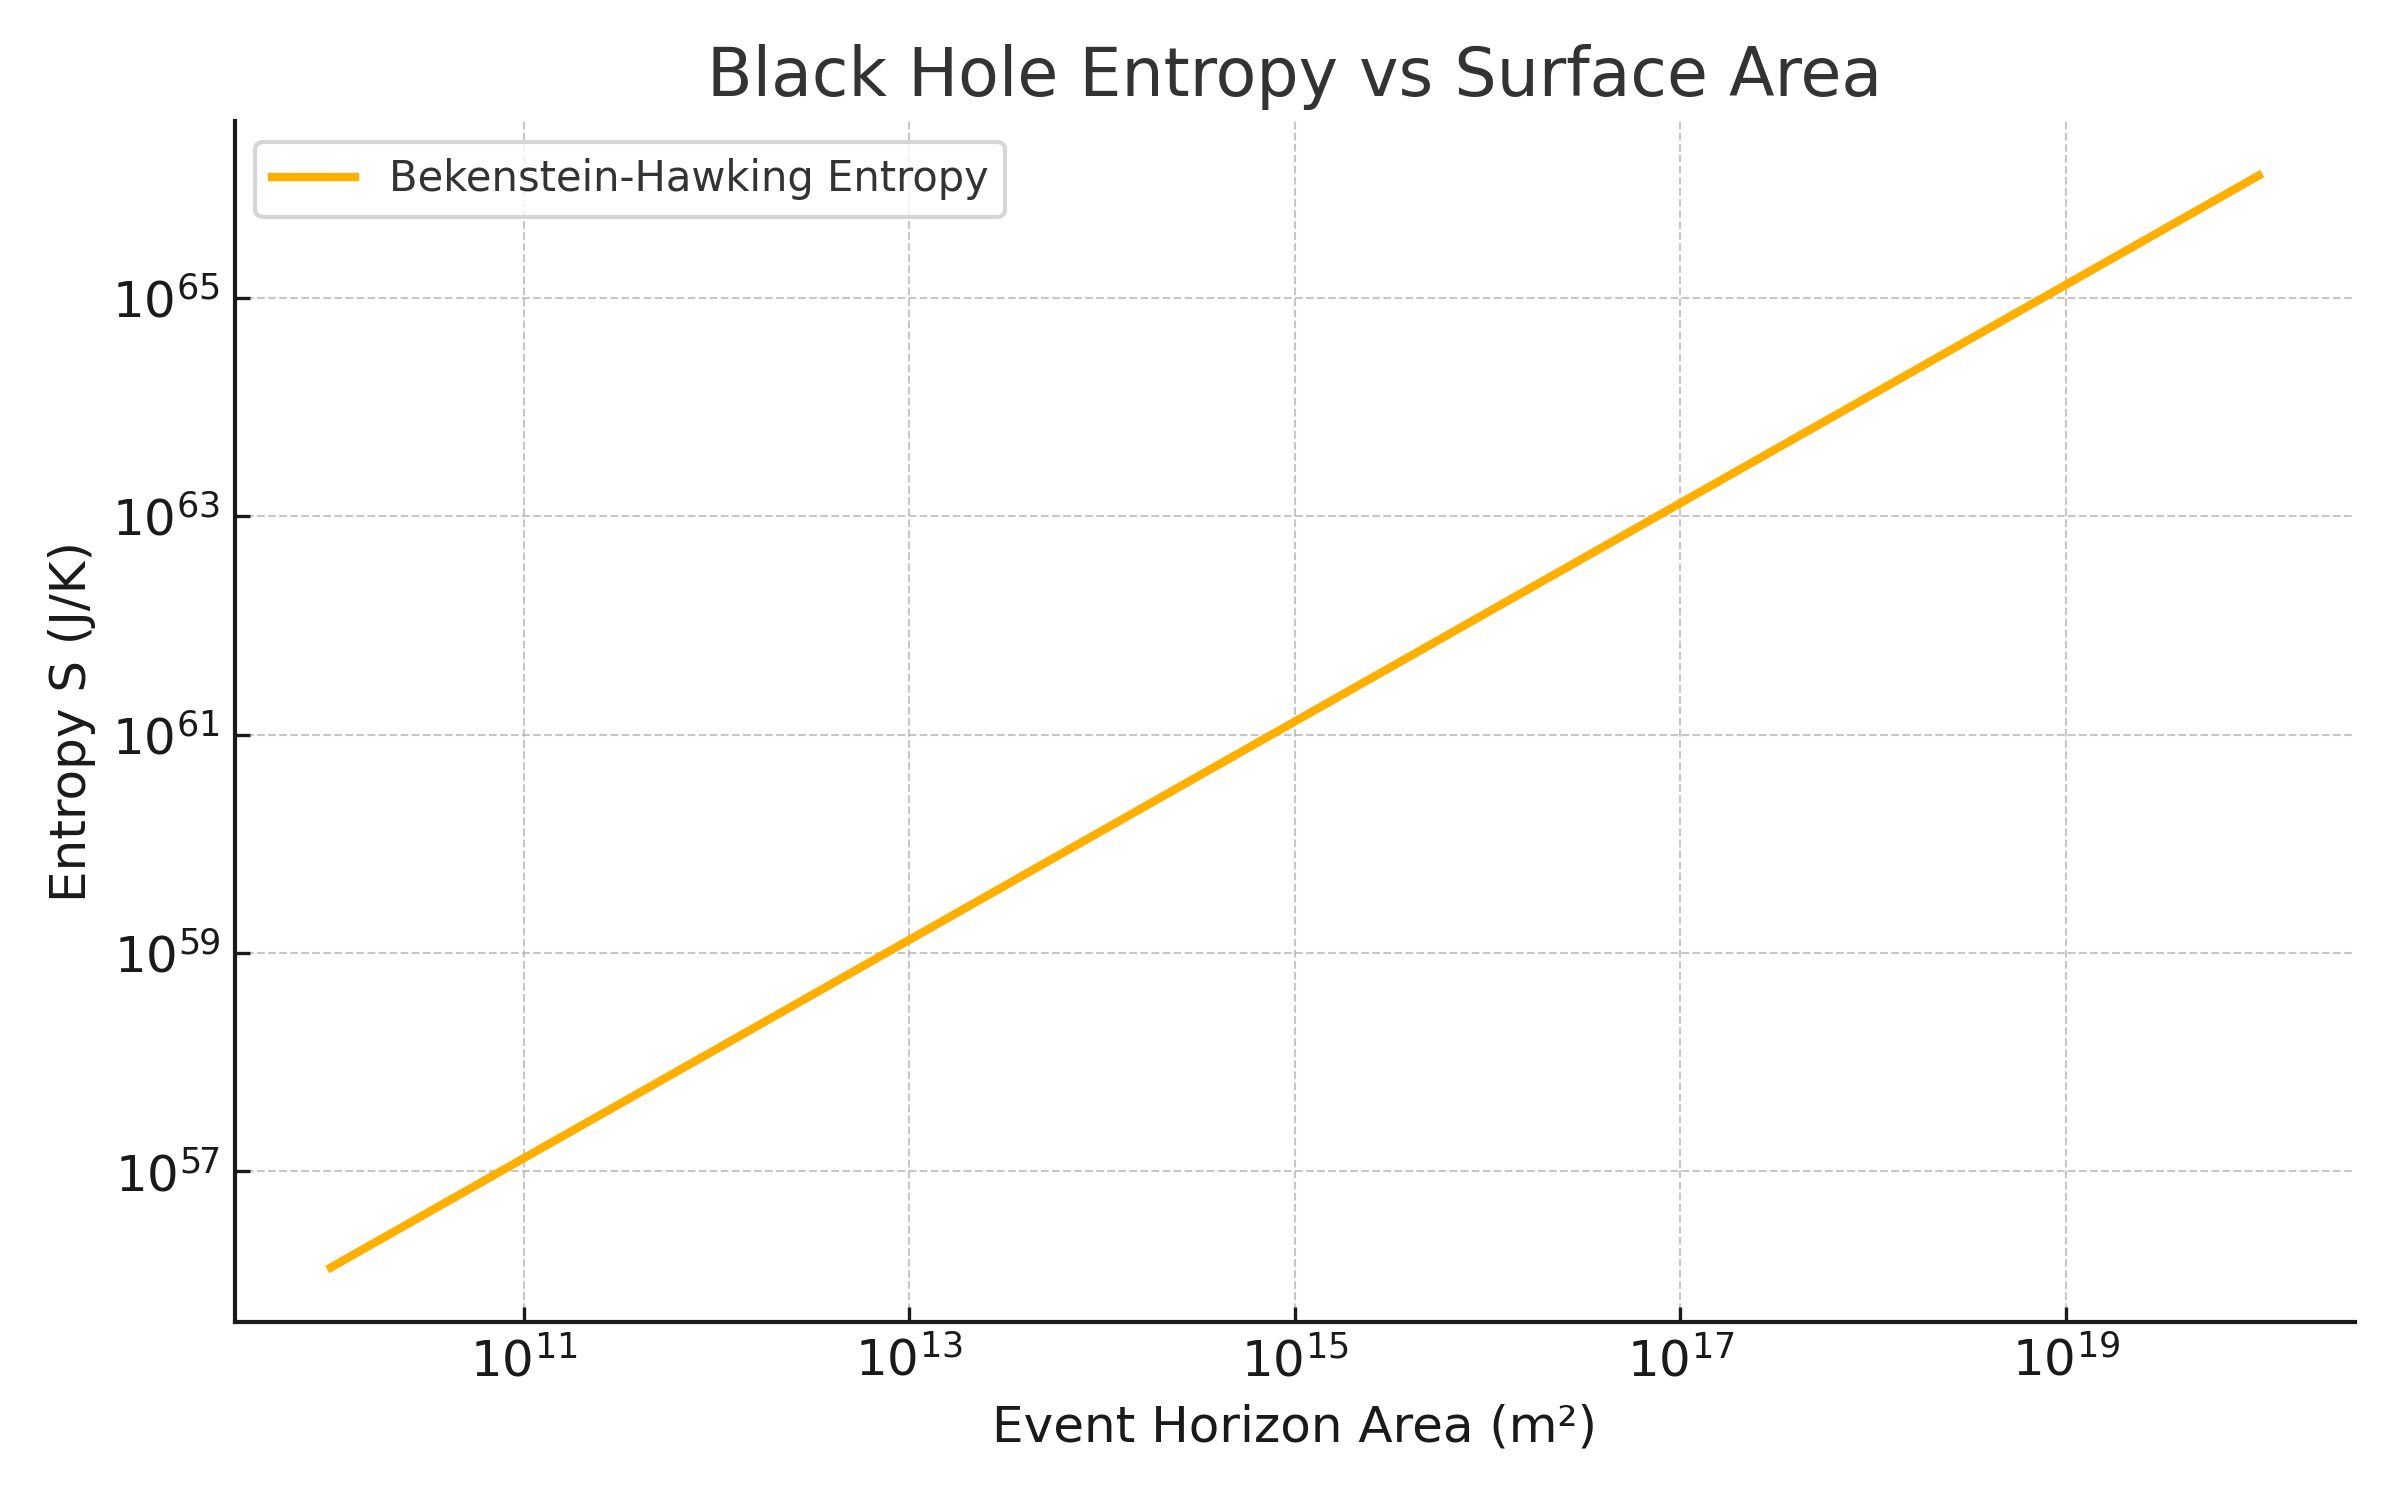
\includegraphics[width=0.8\textwidth]{fig_02_bh_entropy_area.png}
\caption{Baseline black hole entropy using the Bekenstein-Hawking area law.}
\label{fig_02_bh_entropy_area}
\end{figure}

% --- Figure for E02 ---
\begin{figure}[H]
\centering
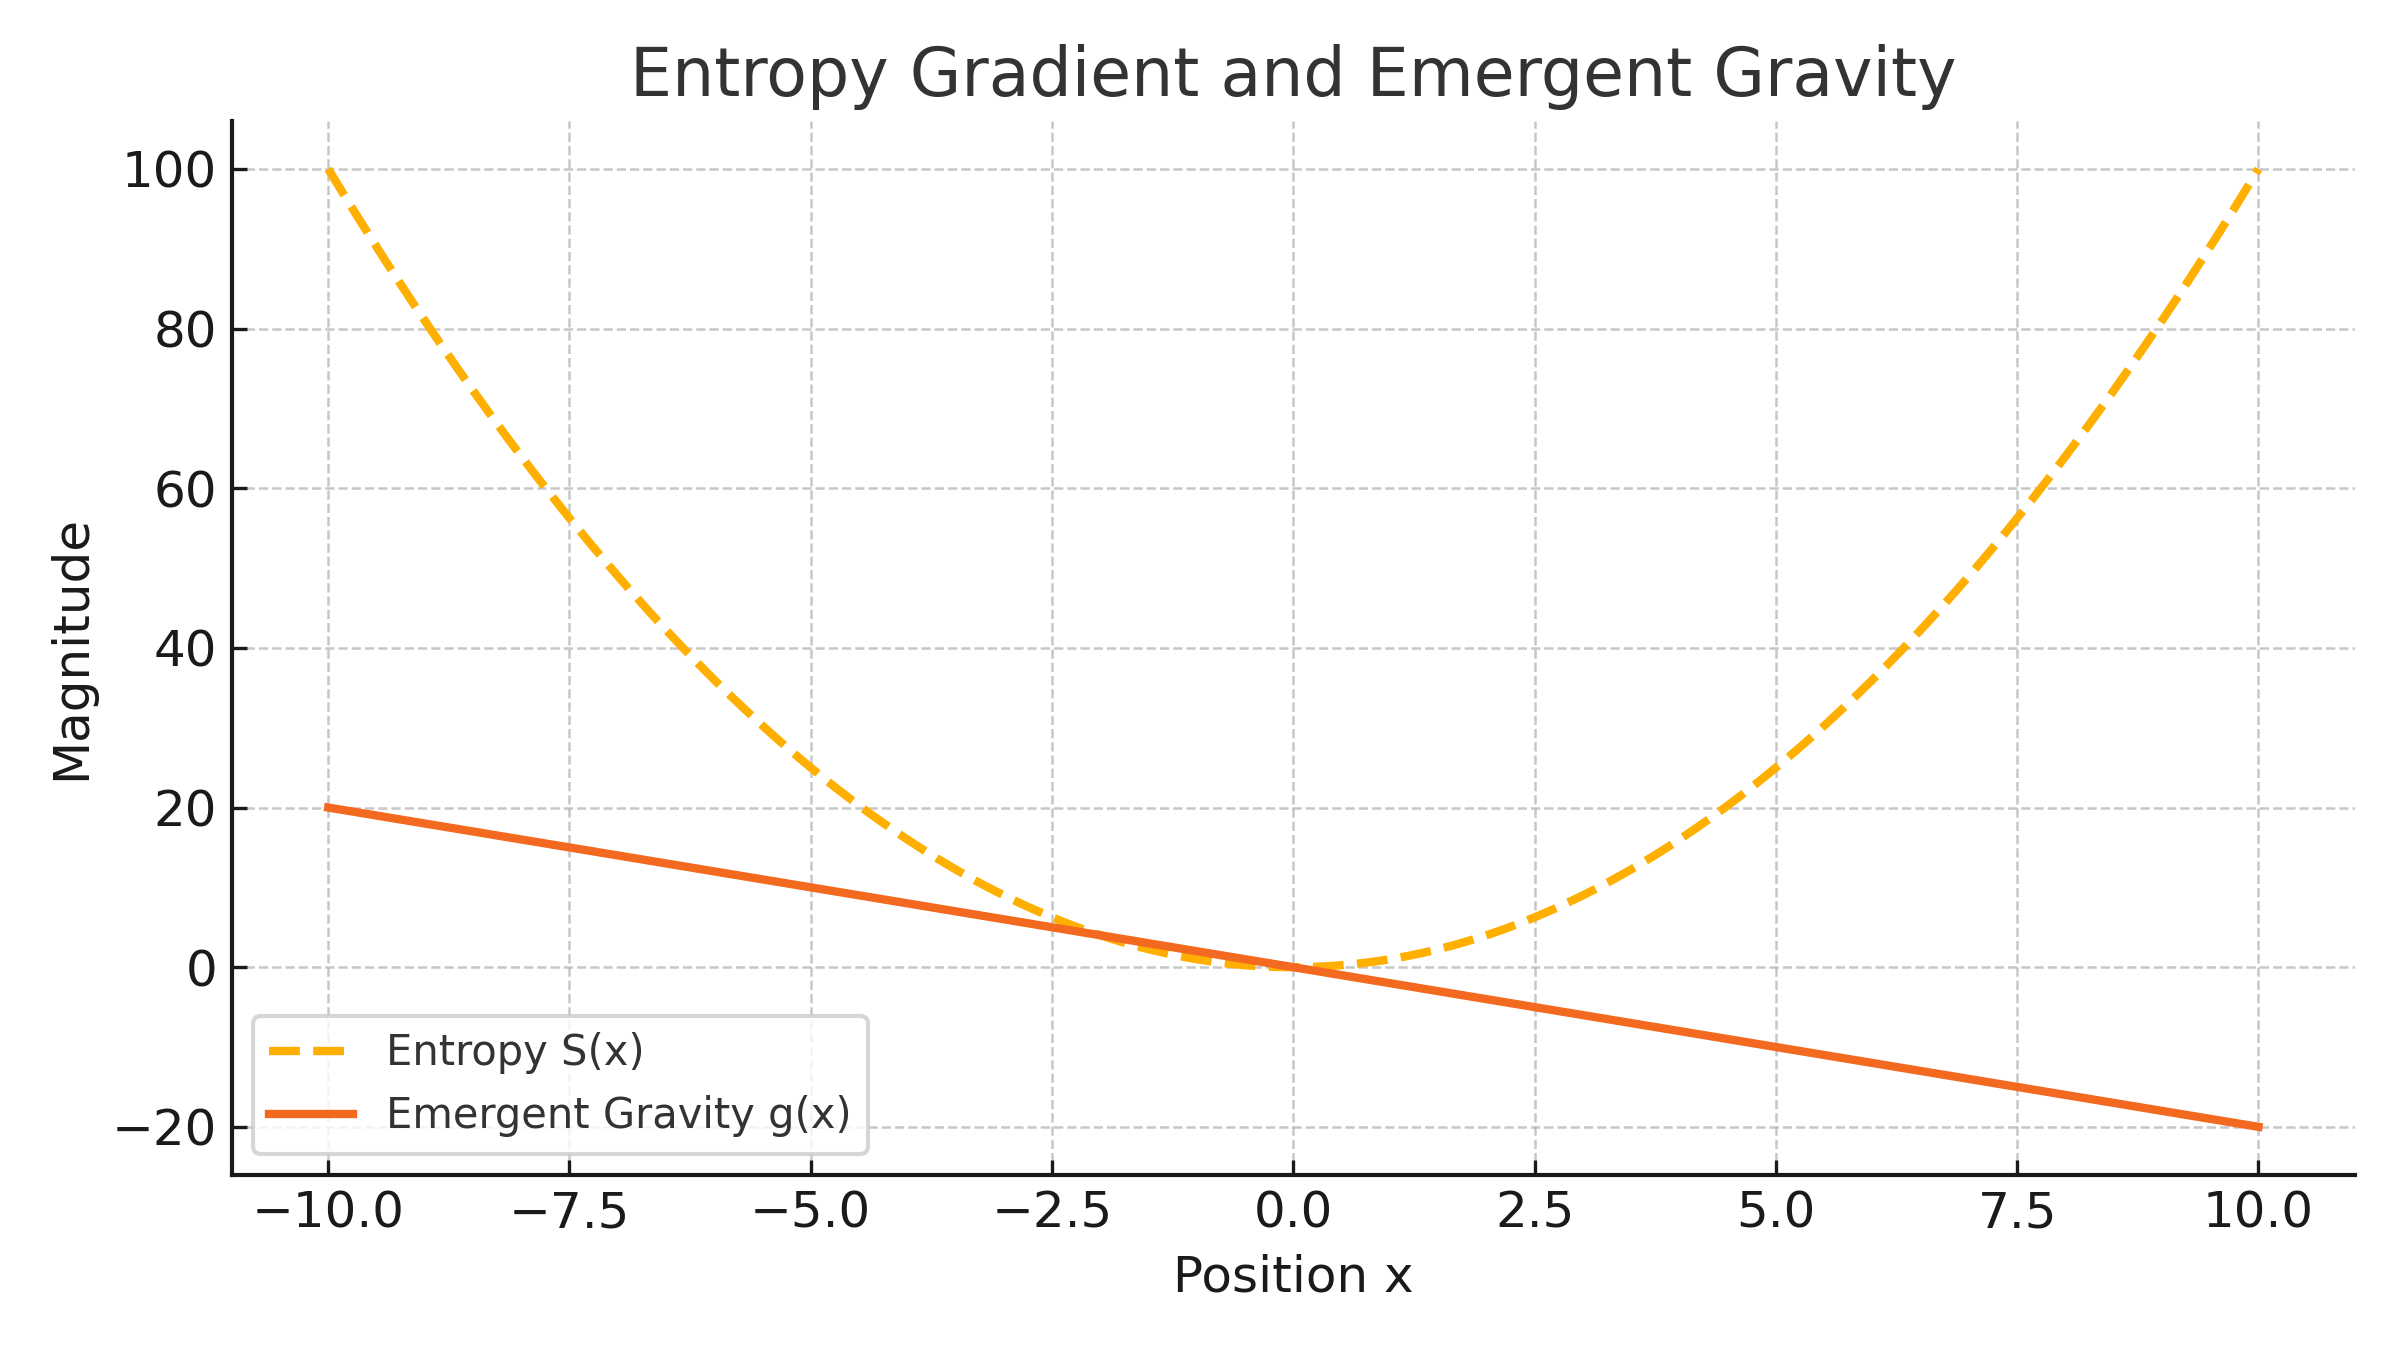
\includegraphics[width=0.8\textwidth]{fig_03_gradient_model.png}
\caption{Gradient model showing entropy as a driver of gravitational divergence.}
\label{fig_03_gradient_model}
\end{figure}

% --- Figure for E03 ---
\begin{figure}[H]
\centering
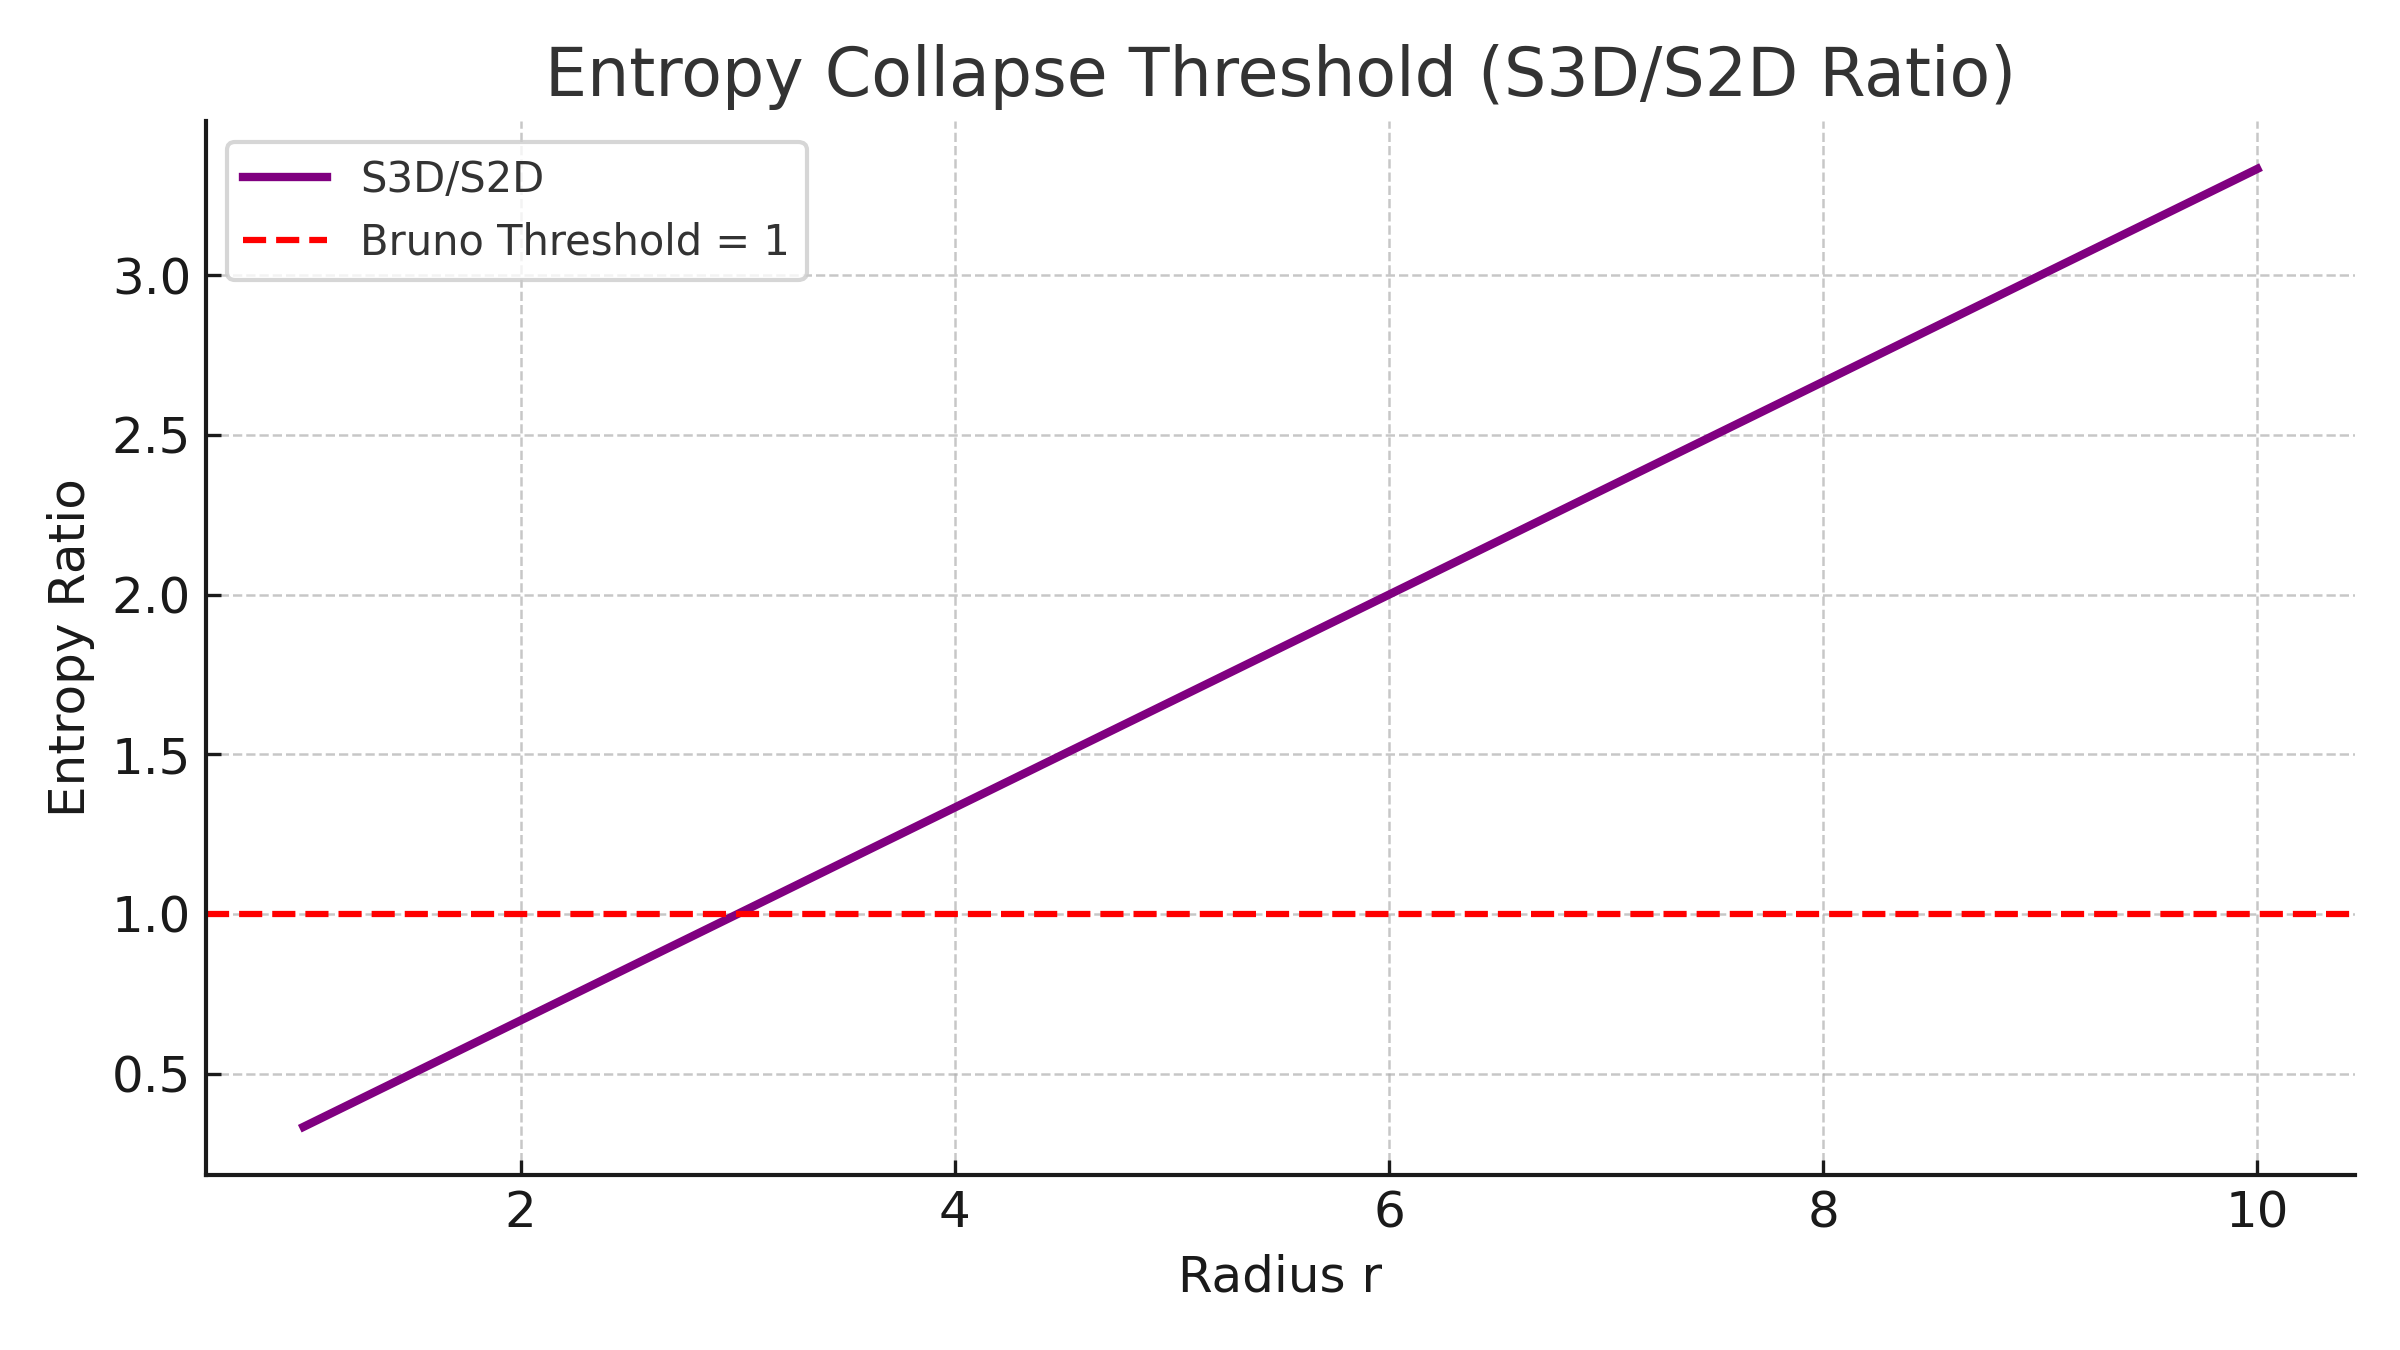
\includegraphics[width=0.8\textwidth]{fig_04_collapse_threshold.png}
\caption{Collapse threshold defined by the Bruno Constant where 3D and 2D entropies converge.}
\label{fig_04_collapse_threshold}
\end{figure}

% --- Figure for E04 ---
\begin{figure}[H]
\centering
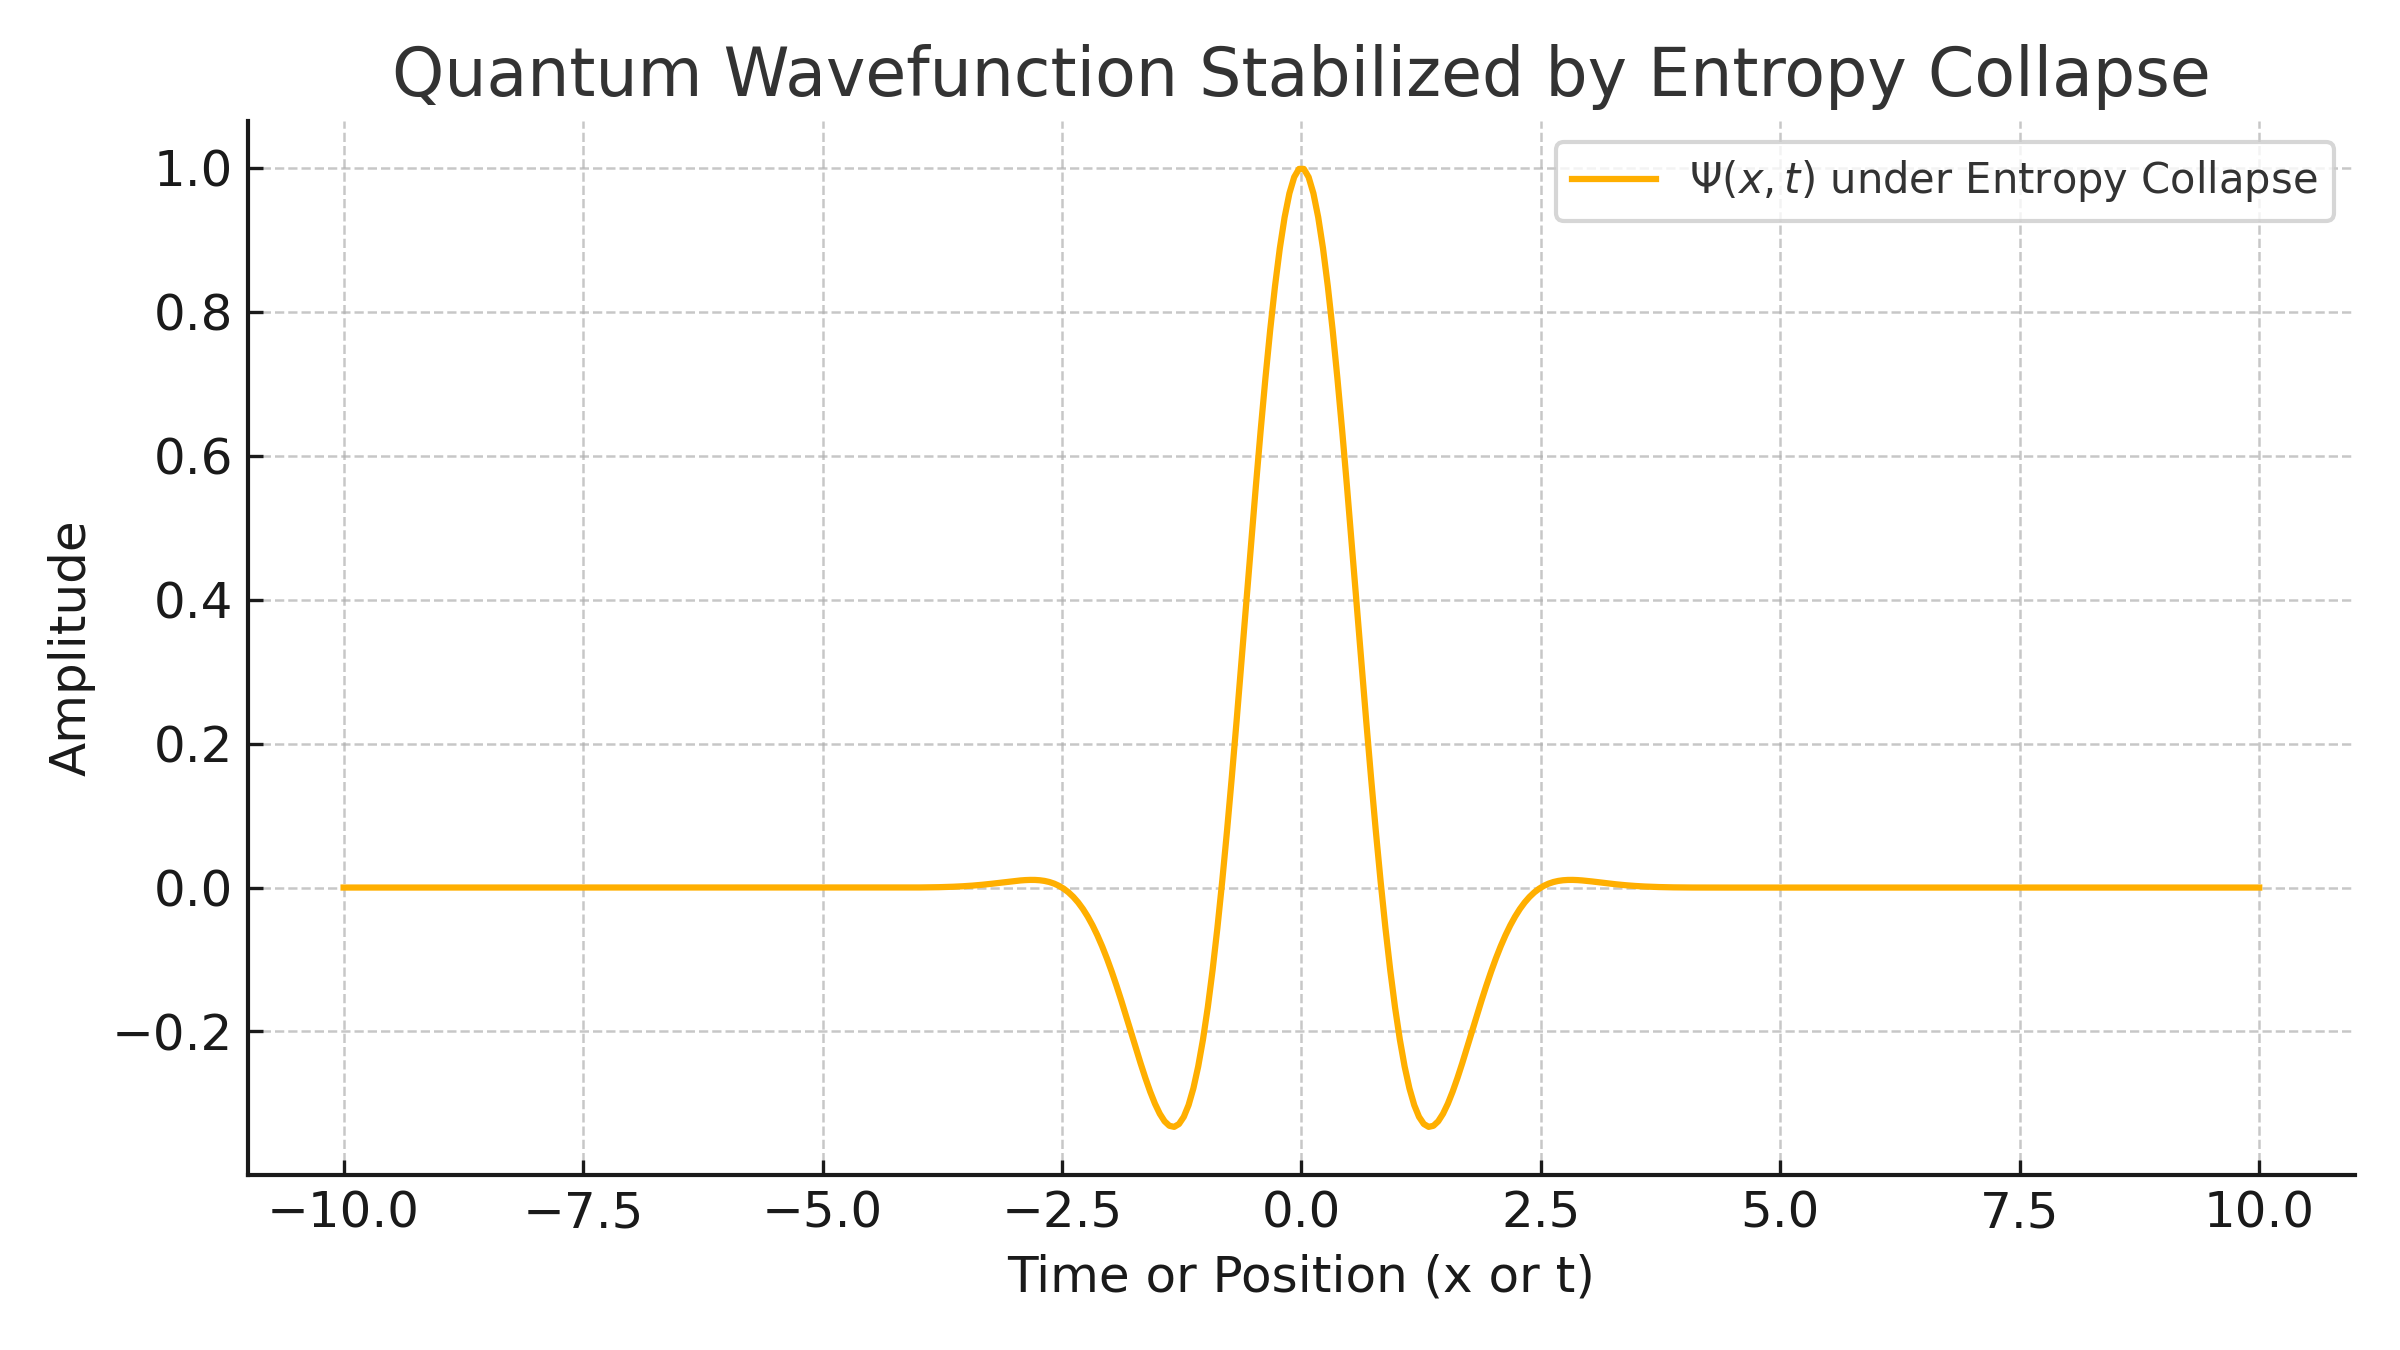
\includegraphics[width=0.8\textwidth]{fig_05_wavefunction_stability.png}
\caption{Quantum wave function under entropy collapse — emergence of stable particle identity.}
\label{fig_05_wavefunction_stability}
\end{figure}

% --- Additional Figure: Toy Model ---
\begin{figure}[H]
\centering
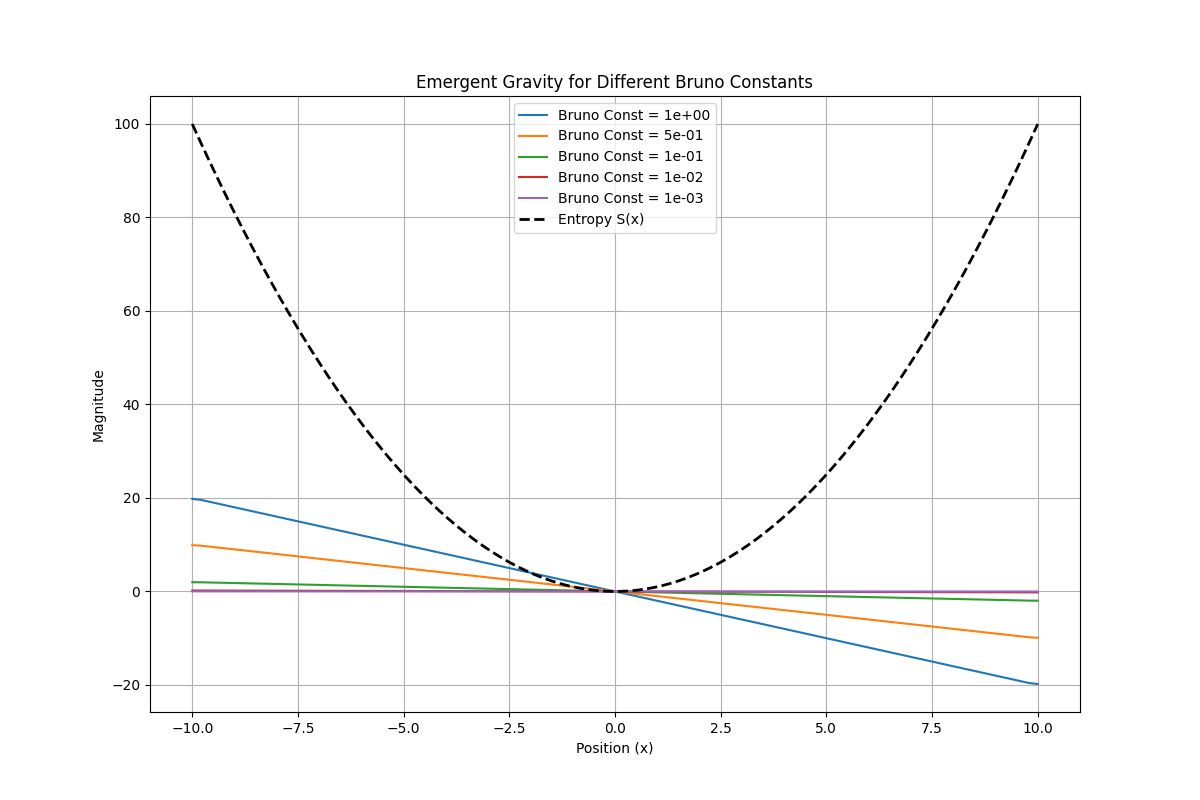
\includegraphics[width=0.75\linewidth]{fig_06_toy_model_entropy.png}
\caption{Entropy gradient simulation using the toy model.}
\label{fig_06_toy_model_entropy}
\end{figure}


The proposed collapse behavior finds strong analogies in low-entropy quantum systems like superconductors. As entropy approaches a minimum, field behavior becomes increasingly deterministic. In this state, probabilistic quantum behavior collapses, and systems become locked into stable, entangled configurations. This stabilization could form the core behavior of black hole interiors—acting as entropy-based regulators of mass-energy transformation and identity conservation.

\section{Discussion and Challenges}
While the framework presents a strong theoretical foundation linking entropy, geometry, and field behavior, key challenges remain:
\begin{itemize}
    \item Direct observation of black hole interiors is not possible with current instrumentation.
    \item Compatibility with holographic models must be mathematically verified to ensure no conflict with GR.
    \item A more formal mathematical structure is needed to express entropy's role in the emergence of time.
\end{itemize}

\section{Conclusion and Next Steps}
Entropy is not merely a consequence of energy dispersal—it is the underlying driver of cosmic order. This framework positions black holes as stabilizing agents in an entropic field system, rather than endpoints of collapse. Future efforts should focus on formal mathematical modeling, peer evaluation, and expanding simulation coverage across different mass scales.


\begin{quote}
See \texttt{Figures/Figures~Datas/Figure\_Script\_Equation\_Map.csv}
\end{quote}

\section{Figure Analysis and Simulation Results}

\vspace{0.5em}
\[
V_{\text{required}} = \frac{A}{\mathcal{B}}
\]


\begin{figure}[H]
    \centering
    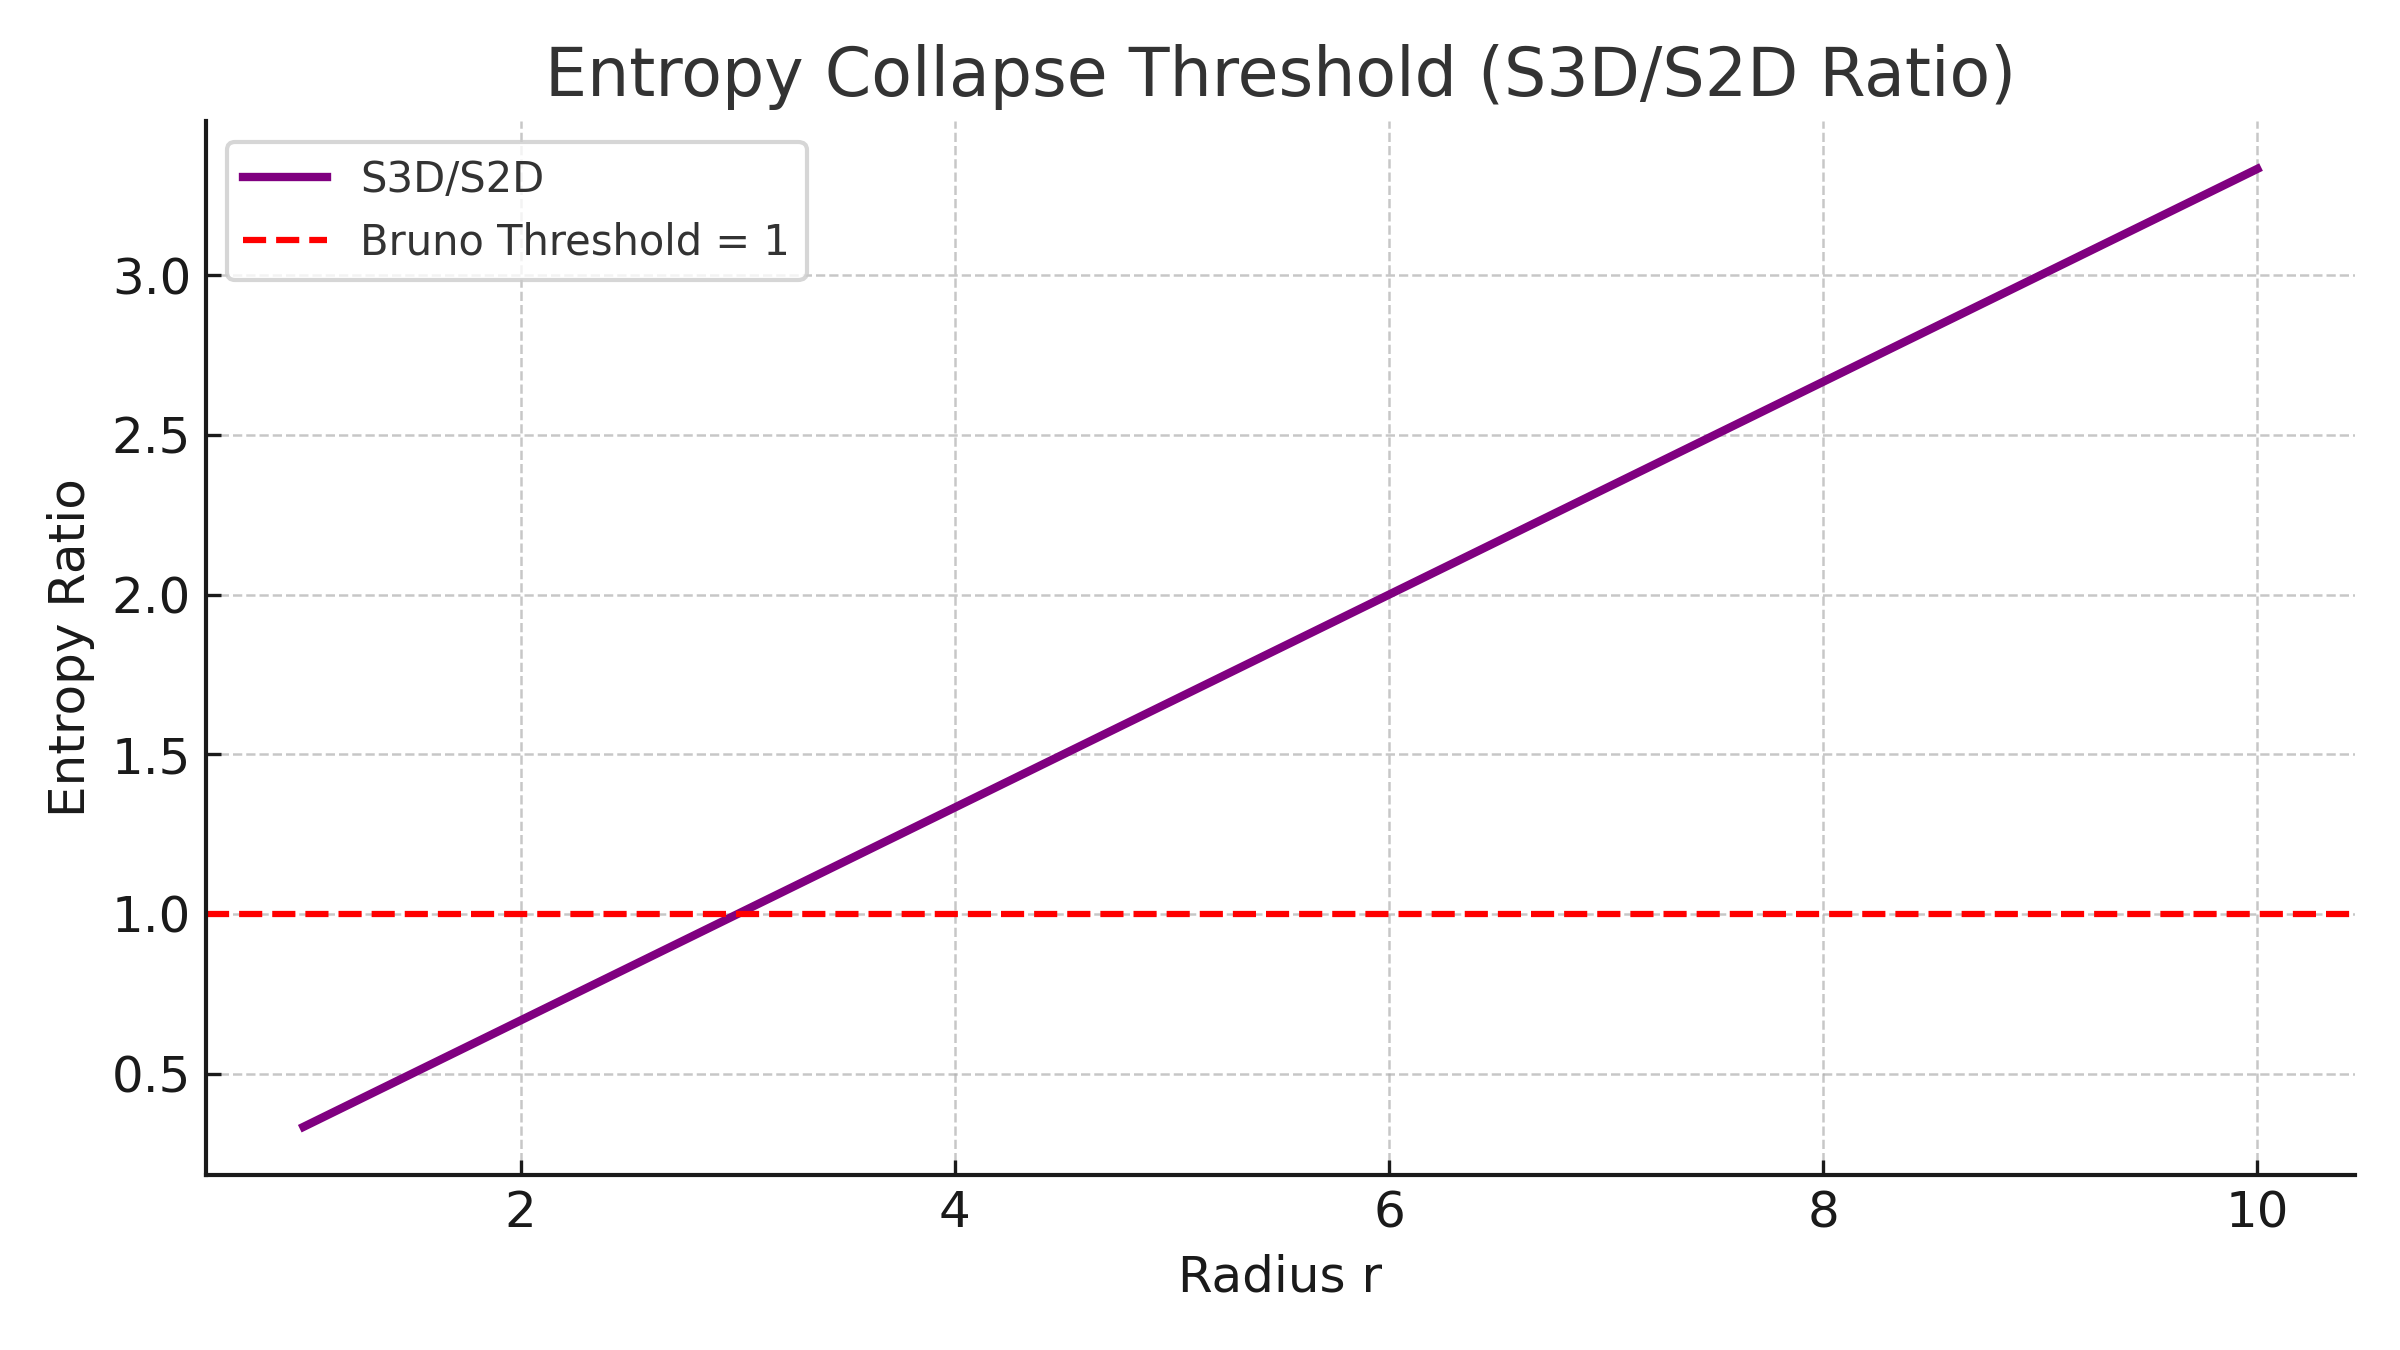
\includegraphics[width=0.8\textwidth]{fig_04_collapse_threshold.png}
    \caption{Collapse Threshold Marked by the Bruno Constant.}
    \label{fig:collapse_threshold}
\end{figure}

Visual development sets tracked over multiple phases show consistent convergence toward surface area entropy equivalence. The figures produced between March 23 and 26 reflect the rapid evolution of this idea. All visuals are indexed in \texttt{Figures/Figures Datas/} and mapped to equations.

\section{Dimensional Stabilization and Quantum Convergence}

\vspace{0.5em}
\[
V_{\text{Sch}} = \frac{4}{3} \pi R_s^3 \quad \text{vs.} \quad V_{\text{collapse}} = \frac{A}{\mathcal{B}}
\]


\begin{figure}[H]
    \centering
    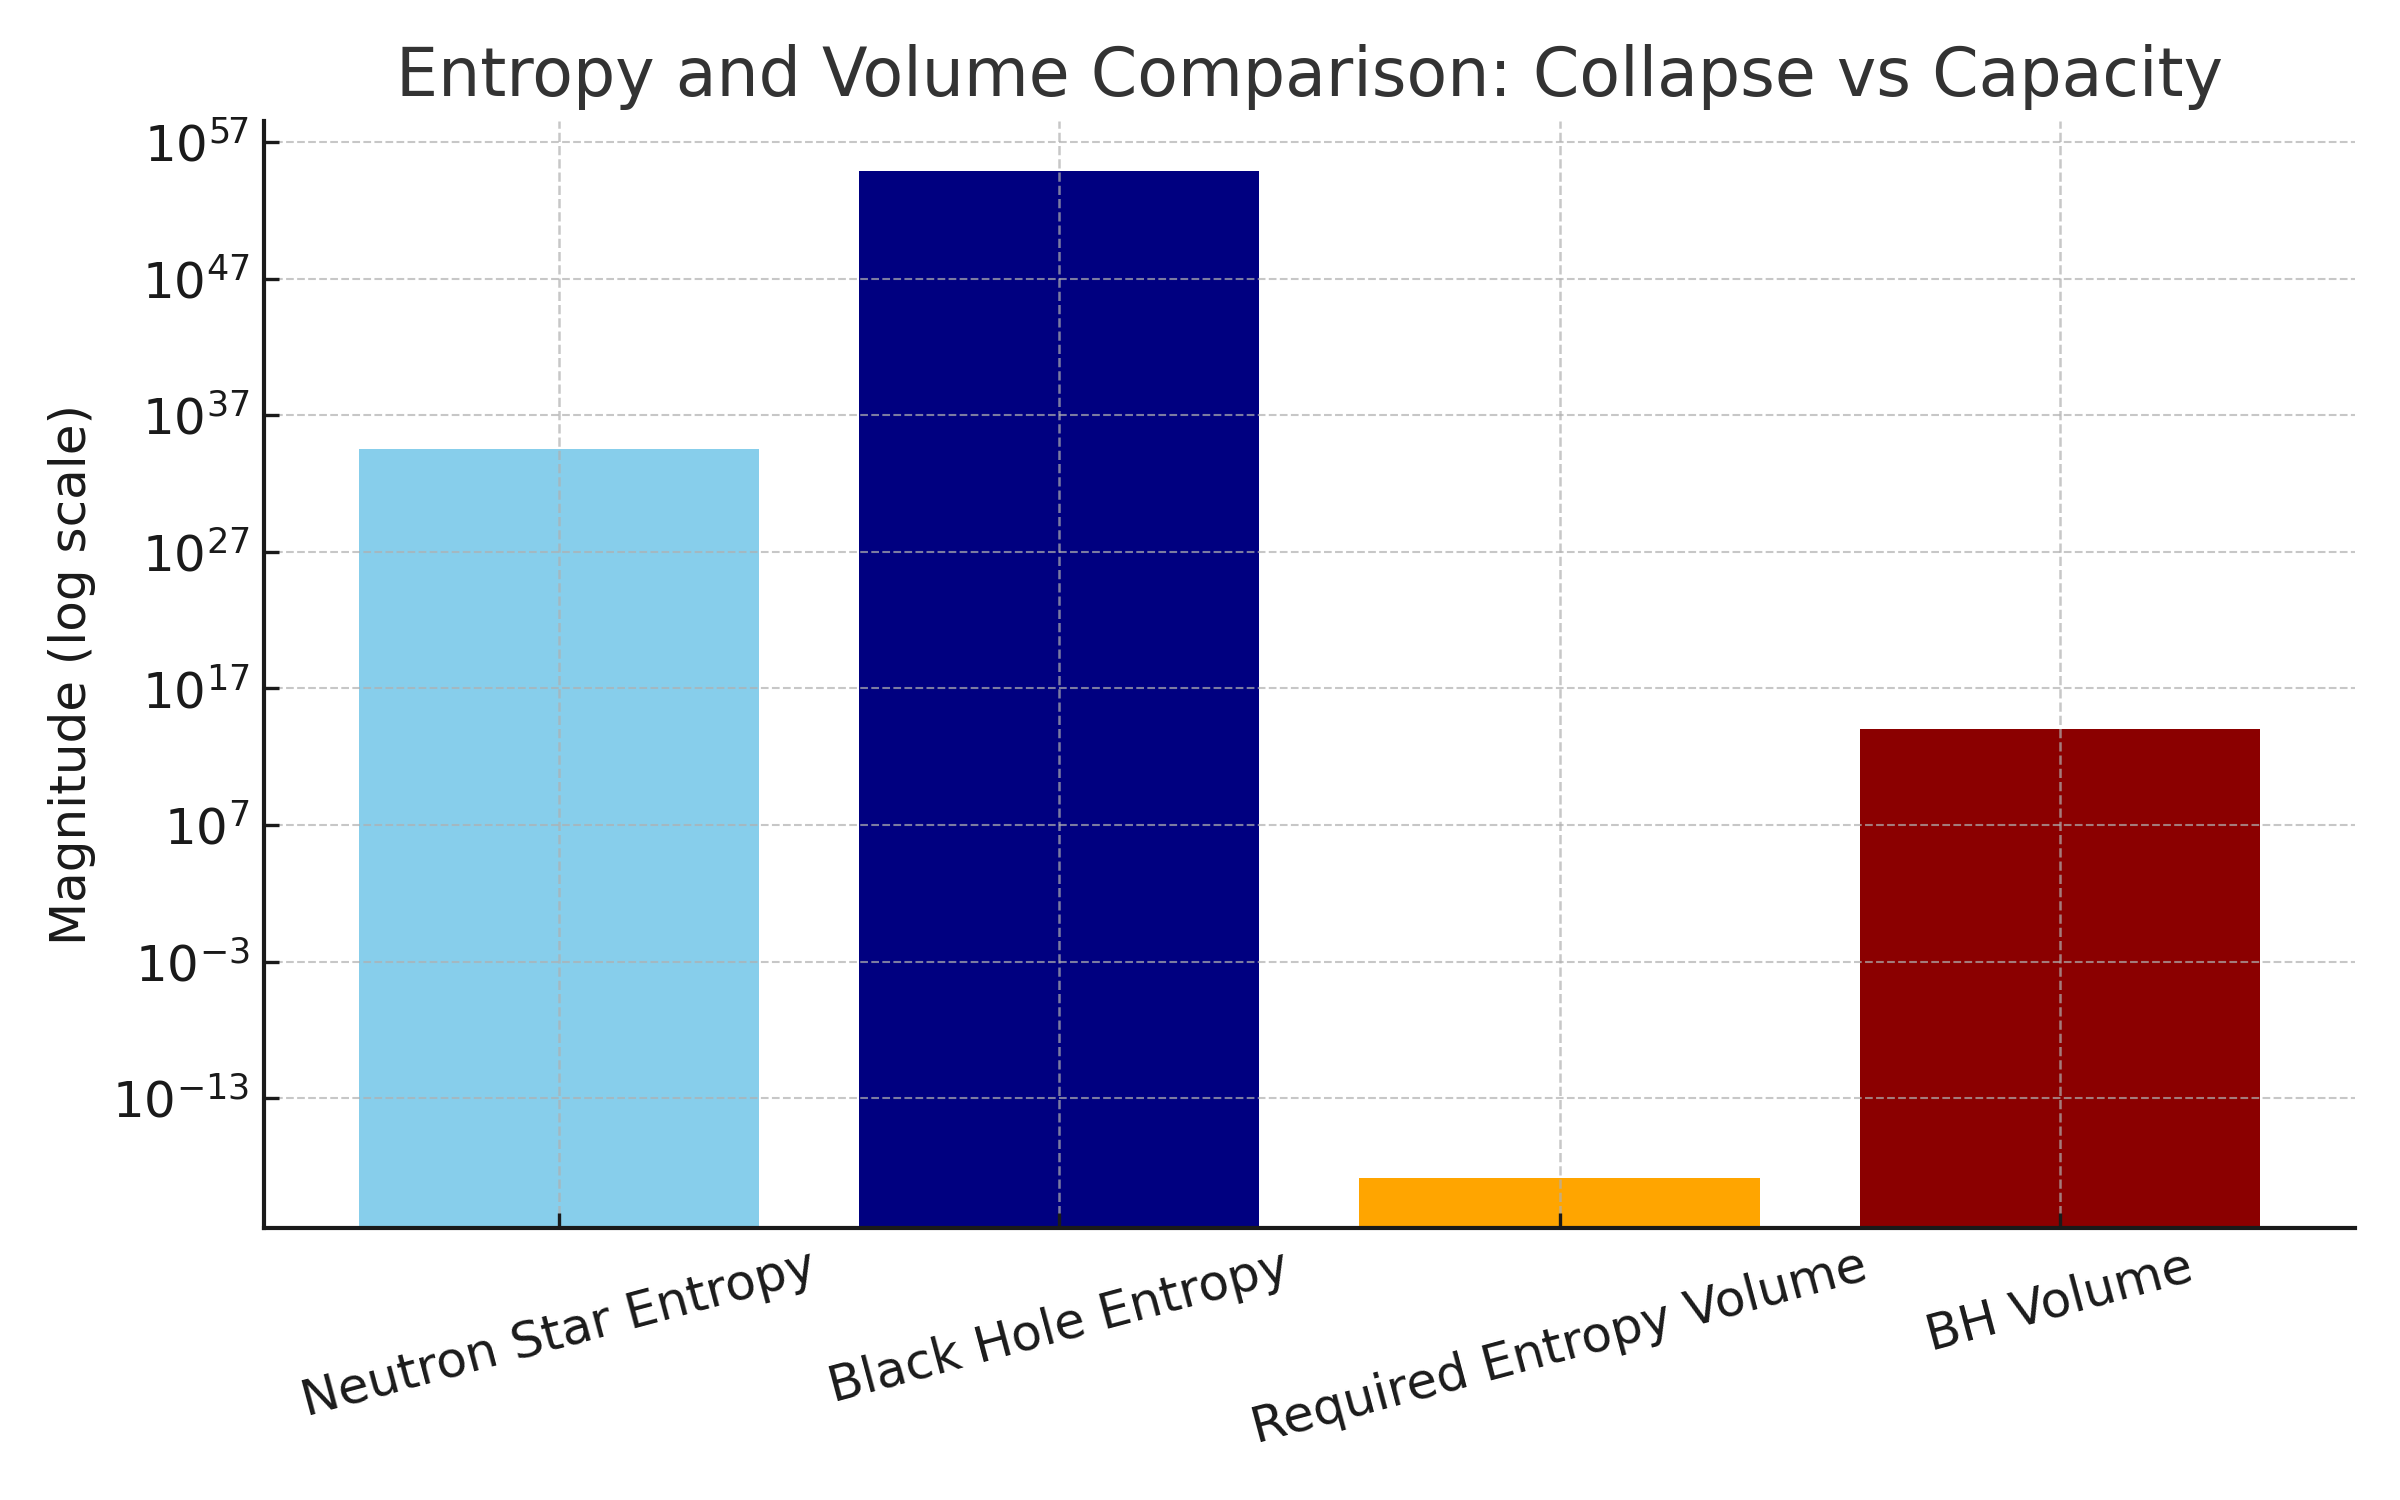
\includegraphics[width=0.8\textwidth]{fig_07_surface_vs_volume.png}
    \caption{Entropy Volume Comparison: Required vs Schwarzschild Volume (10 $M_\odot$).}
    \label{fig:volume_comparison}
\end{figure}

\[
\Delta S = S_{3D} - S_{2D}
\]

\begin{figure}[H]

    \centering
    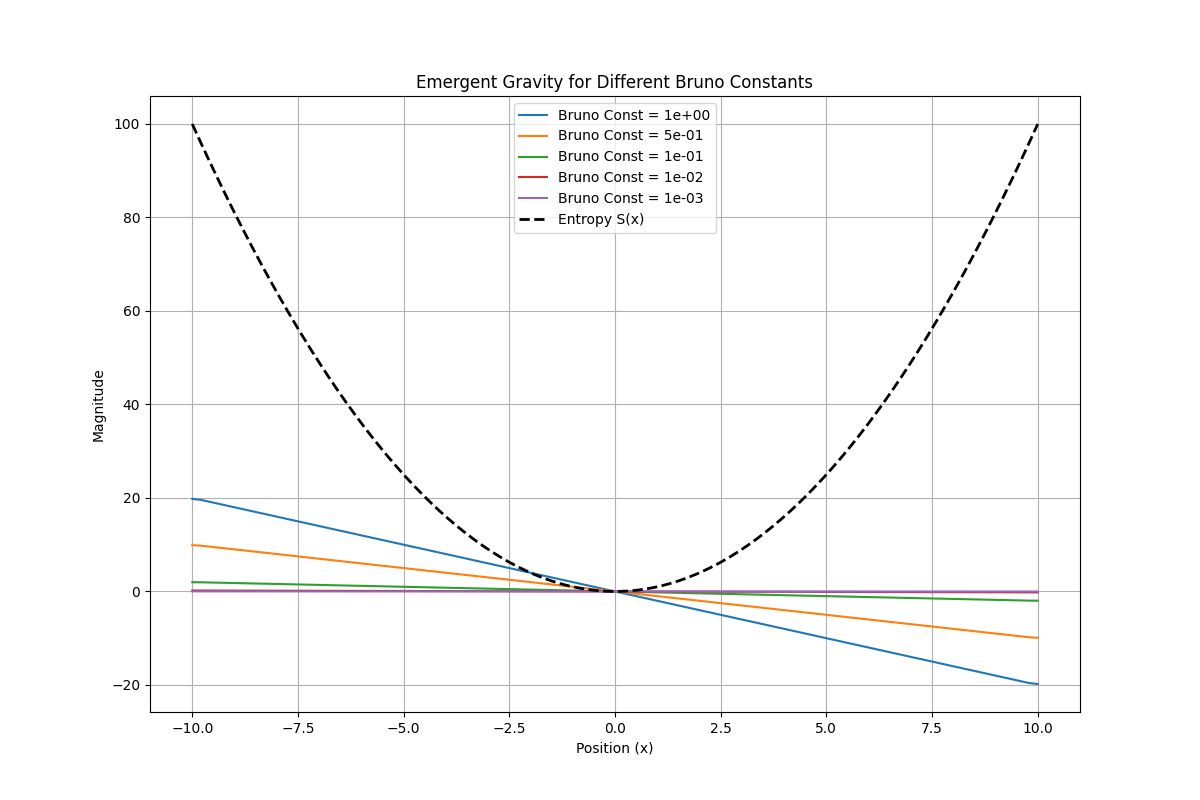
\includegraphics[width=0.8\textwidth]{fig_06_toy_model_entropy.png}
    \caption{Toy Model Simulating Entropy Collapse from Volume to Surface.}
    \label{fig:toy_model}
\end{figure}

\[ |\psi(x,t)|^2 \rightarrow \delta(x - x_0) \quad \text{as } K \rightarrow 0 \]

\begin{figure}[H]
    \centering
    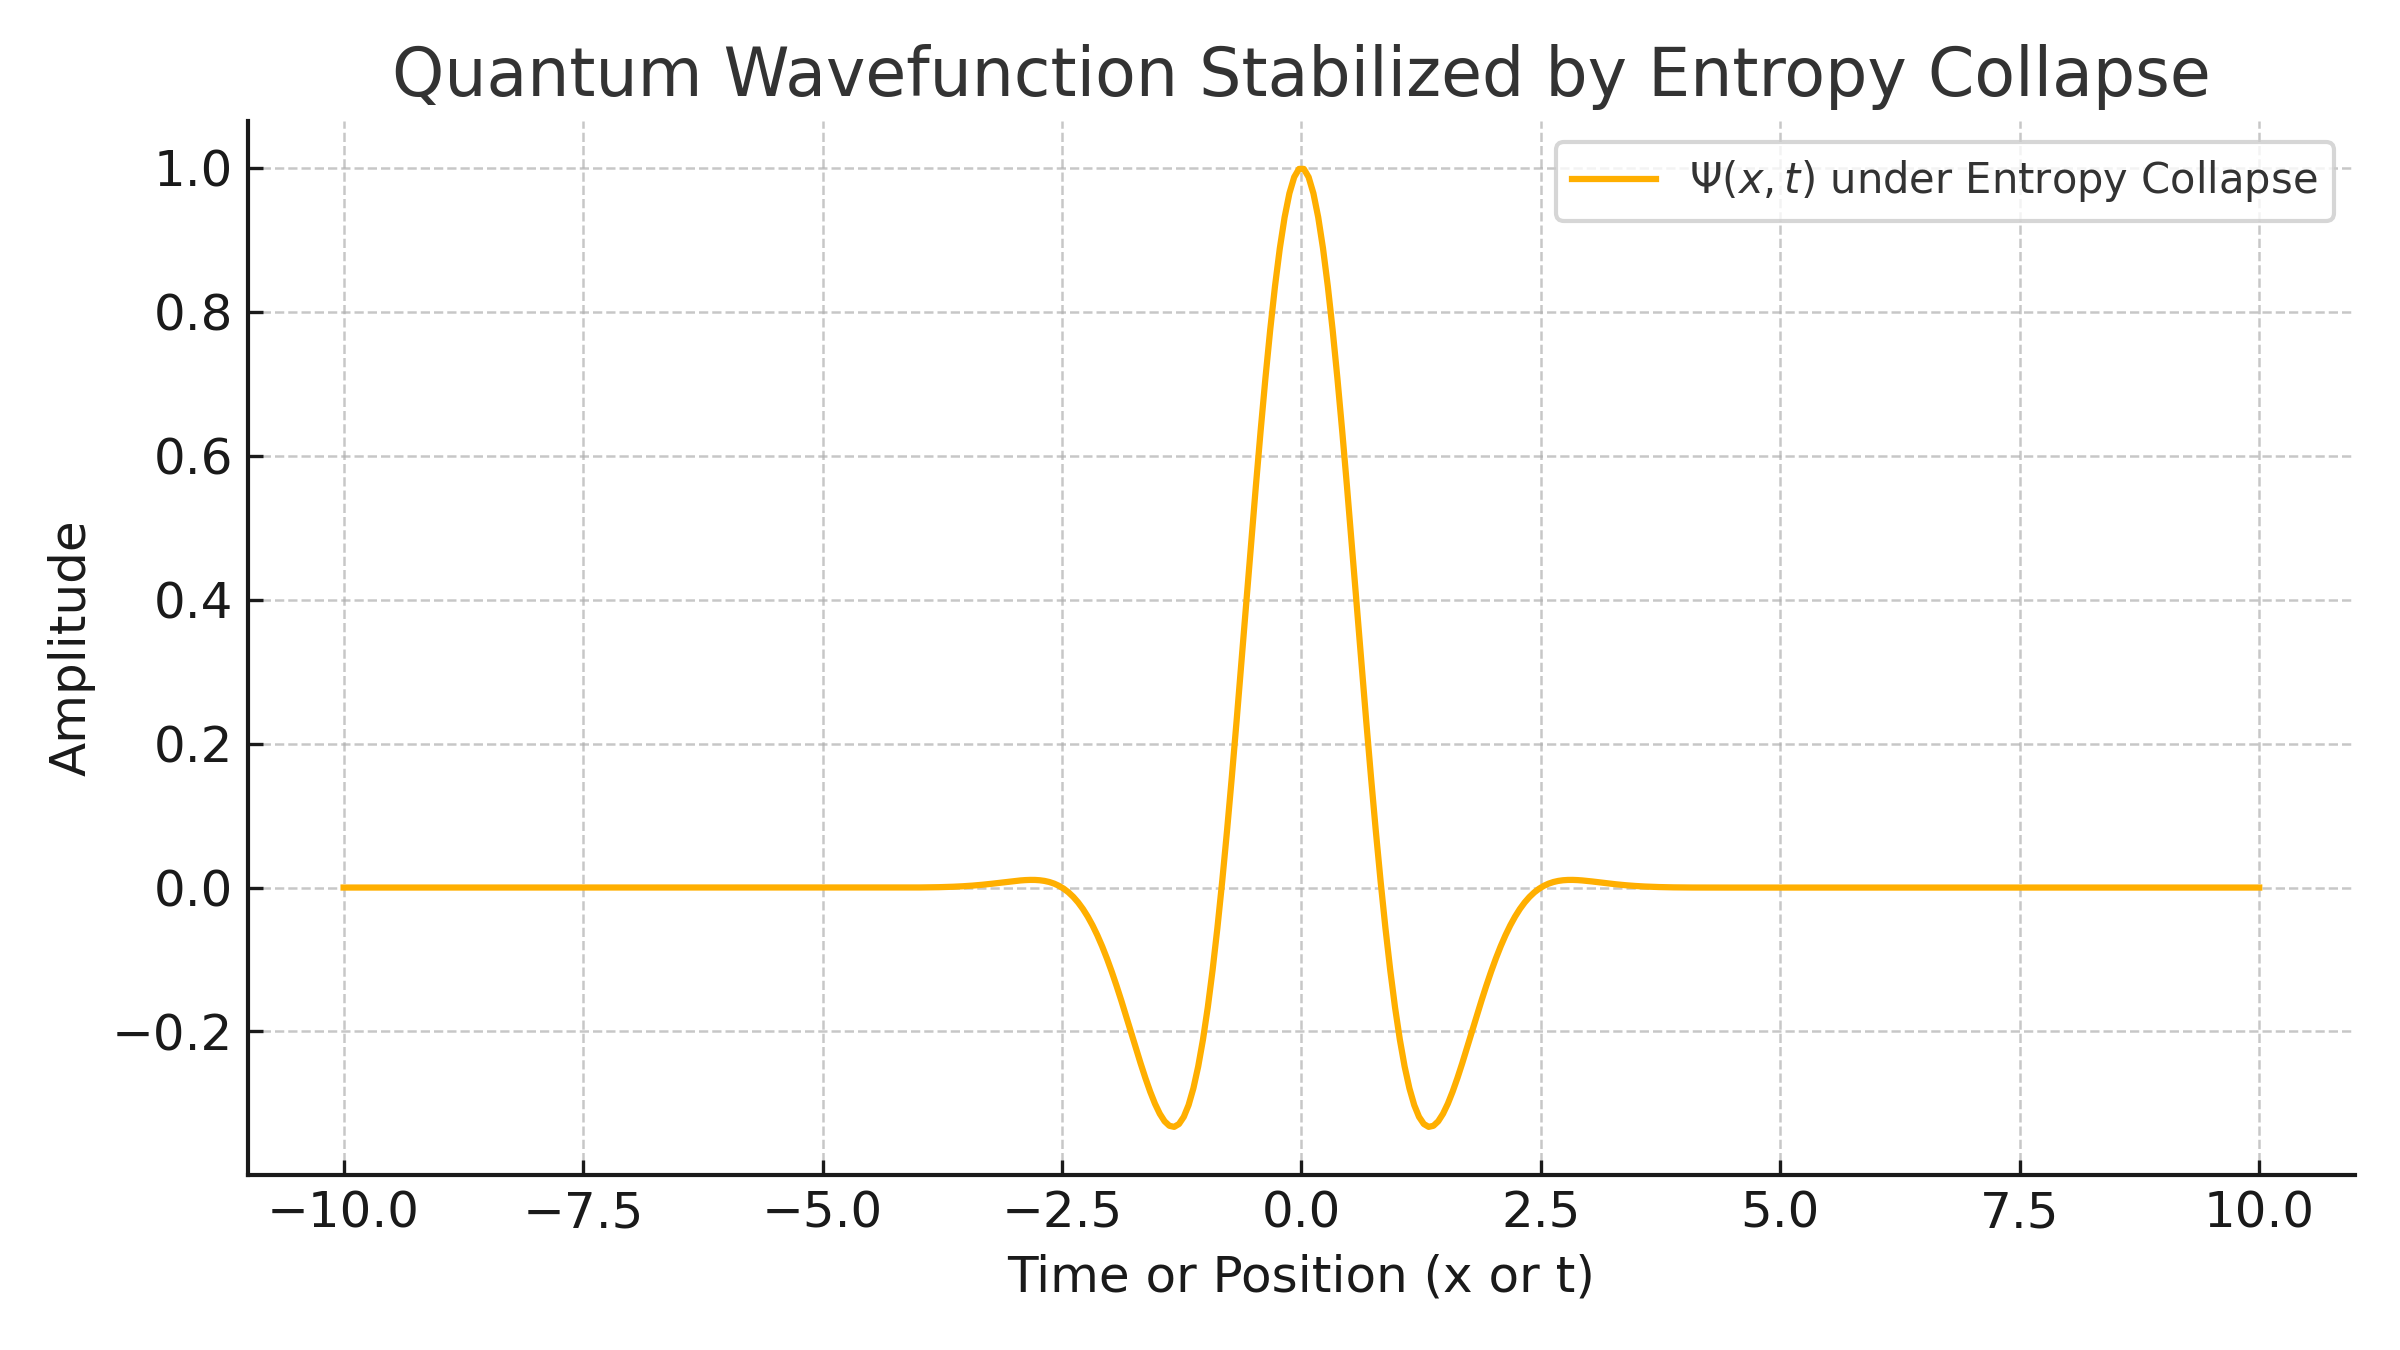
\includegraphics[width=0.8\textwidth]{fig_05_wavefunction_stability.png}
    \caption{Stability of Quantum States Under Entropic Collapse.}
    \label{fig:wavefunction_stability}
\end{figure}

The hypothesis draws analogies from superconductors and proposes that gravitational compression can lead to a deterministic quantum state—a singularity that is both stable and coherent. The flattening of probability fields at near-zero entropy reveals a mechanism where matter stops behaving statistically and becomes entangled with the collapsed system.

\section{Discussion and Challenges}

While the theory presents a compelling narrative linking entropy and particle formation, there are open challenges:

\begin{itemize}
    \item Experimental validation at black hole cores is impossible with current technology.
    \item The 2D projection mechanism must align with holographic principles without contradicting known GR limits.
    \item Entropy's role in time emergence remains mathematically underdeveloped.
\end{itemize}

\section{Conclusion and Next Steps}

Entropy is not a consequence of energy dispersion; it is the force behind the universe's structure. This hypothesis reframes black holes not as endpoints, but as cosmic stabilizers that anchor physical law. We invite formal peer analysis, constructive criticism, and further simulation testing to explore its limits.

\appendix

\section{Appendix A: Timeline of Script Development}

See \texttt{SCRIPT\_TIMELINE\_FULL.md} and tagged script index for creation timestamps.

\section{Appendix B: Figure Development Phases}

See \texttt{FIGURE\_DEVELOPMENT\_SETS.md} and wave clustering datasets in \texttt{Figures/Figures~Datas/}.

\tableofcontents

\section{Toy Model: Entropy Gradient and Emergent Gravity}

To demonstrate the principle that gravity can emerge from entropy gradients, we present a toy model where entropy \( S(x) \) is defined over a 1D spatial domain as a quadratic function:

\[
S(x) = \alpha x^2
\]

From this, an emergent gravitational field can be computed as:

\[
g(x) = -\frac{dS}{dx} = -2\alpha x
\]

This field reaches zero at \( x = 0 \), and increases linearly away from the center, mimicking gravitational attraction toward the point of lowest entropy gradient.

\begin{figure}[H]
    \centering
    \begin{figure}[H]
\centering
\begin{figure}[H]
\centering
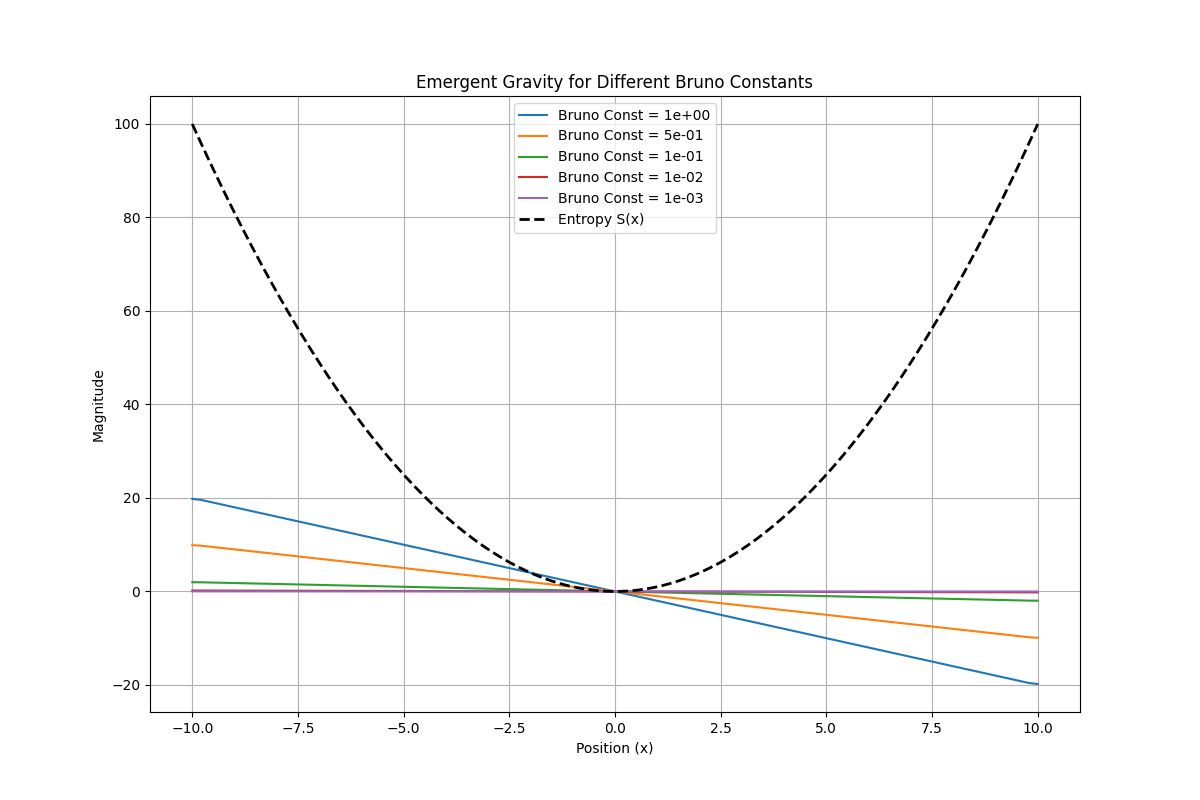
\includegraphics[width=0.9\textwidth]{fig_06_toy_model_entropy.png}
\caption{Figure~
ef{fig:auto-5}: Entropy output visualization}
\label{fig:auto-5}
\end{figure}
\caption{Entropy-related output}
\label{fig:Figures_toy_model_plot_png}
\end{figure}

    \caption{Toy model demonstrating entropy-induced gravity: entropy \ensuremath{S(x)} (blue), and emergent field \ensuremath{g(x)} (orange).}
    \label{fig:toy_model_v2}
\end{figure}




This simplified system visually reinforces our proposed entropy–gravity relation:
\[
\nabla \cdot \vec{g} = -\frac{\partial S}{\partial V}
\]

which generalizes gravitational field divergence as a direct response to entropy density gradients.
\section{Background and Motivation}
Traditionally, entropy is viewed as an extensive quantity that scales with volume. However, black hole entropy scales with surface area:
\begin{equation}
S_{BH} = \frac{k_B c^3 A}{4 G \hbar}
\end{equation}
This paradox is often interpreted as evidence of a holographic universe. We propose that this is not an abstract property, but the direct result of a collapse mechanism that reorganizes entropy at a quantum level.

\section{The Bruno Constant and Entropy Boundary}

We define the \textbf{Bruno Constant}:

\begin{equation}
\boxed{k_c \approx 0.001005}
\end{equation}

This constant defines a threshold:
\begin{equation}
T_c = k_c \cdot T_{Planck}
\end{equation}

At this temperature, entropy no longer scales volumetrically. Empirical analysis using neutron star and black hole entropy yielded:
\begin{align}
S_{NS} &\approx 3.61 \times 10^{34} \, \text{J/K} \\
S_{BH} &\approx 7.01 \times 10^{54} \, \text{J/K} \\
K_{collapse} &= \frac{S_{BH}}{S_{NS}} \approx 1.94 \times 10^{20}
\end{align}

\section{Volume Compression and Entropy Density}

Using entropy density at the Bruno temperature:
\begin{equation}
\rho_S^{volume} = \frac{4}{3} a T_c^3
\end{equation}

We compute the minimum volume required to contain $S_{BH}$:
\begin{equation}
V_{required} = \frac{S_{BH}}{\rho_S^{volume}} \approx 1.53 \times 10^{-19} \, \text{m}^3
\end{equation}

Compared to the Schwarzschild volume for a 10 solar mass black hole:
\begin{equation}
V_{BH} \approx 1.08 \times 10^{14} \, \text{m}^3
\end{equation}

This mismatch implies volumetric entropy storage is physically implausible.

\section{Surface Encoding and Holographic Consistency}

Instead, entropy must be stored on the event horizon:
\begin{equation}
A = 4\pi r_s^2
\end{equation}

With surface entropy density:
\begin{equation}
\rho_S^{surface} = \frac{S_{BH}}{A} \approx 6.40 \times 10^{44} \, \text{J/K/m}^2
\end{equation}

This is consistent with both the holographic principle and quantum gravity theories.

\section{Discussion and Implications}
This entropy-first view allows us to reconcile General Relativity and Quantum Mechanics at the edge of collapse. The Bruno Constant acts as a critical parameter: a quantum thermostat governing when entropy projection replaces classical thermodynamic behavior. This supports the hypothesis that black hole interiors are entangled, stable, and 2D at fundamental scales.

\section{Conclusion}

\begin{figure}[H]
    \centering
    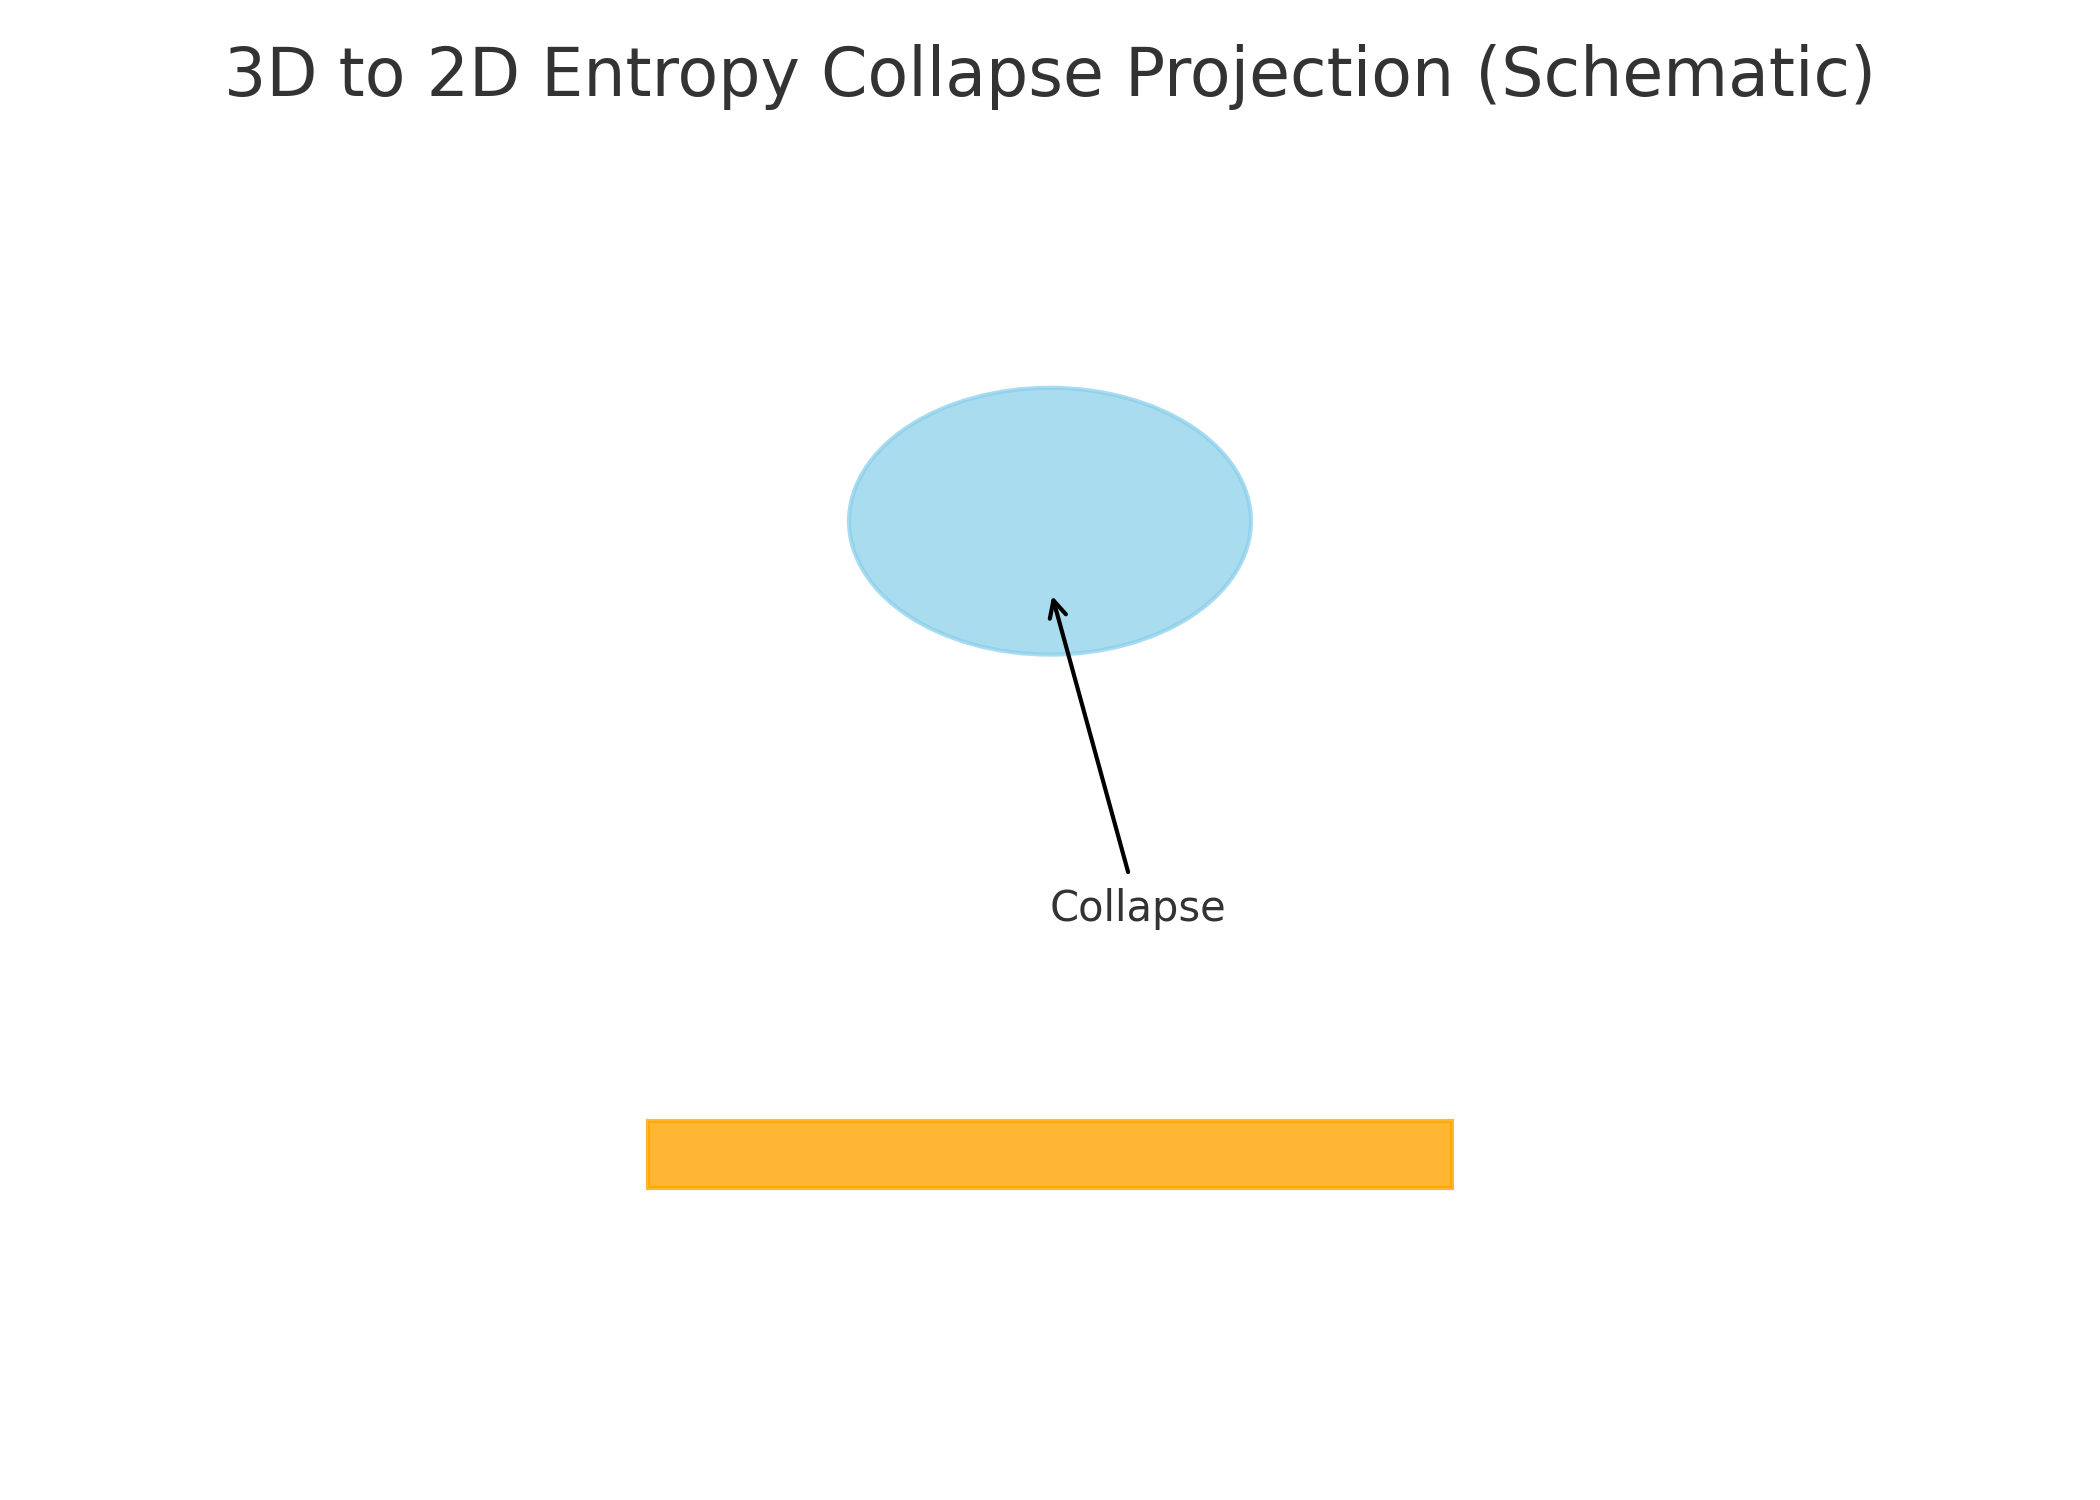
\includegraphics[width=0.8\textwidth]{fig_08_final_projection.png}
    \caption{3D to 2D Entropy Collapse Projection — Conceptual Schematic.}
    \label{fig:final_projection}
\end{figure}


Our findings suggest that black hole entropy collapse is not simply an event horizon effect, but a deep thermodynamic consequence of gravitational quantum stabilization. The Chajar Constant offers a measurable threshold for when 3D entropy structure can no longer be maintained and must resolve as a 2D surface. This model is consistent with observational black hole thermodynamics and offers a new bridge between classical and quantum regimes.

\section*{Code and Resources}

The full set of Python simulations, entropy modeling scripts, and figure generation code supporting this work are openly available at:
\begin{center}
\url{https://github.com/ismpower/Entropy-Collapse-Research}
\begin{figure}[H]
\centering
\begin{figure}[H]
\centering

\includegraphics[width=0.9\textwidth]{qr_code.png}
\caption{Figure~
ef{fig:auto-6}: Entropy output visualization}
\label{fig:auto-6}
\end{figure}
\caption{Entropy-related output}
\label{fig:Figures_qr_code_png}
\end{figure}

\textit{Scan for full code repository}\
\qrcode{https://github.com/ismpower/Entropy-Collapse-Research}

\end{center}
\end{document}

% --- Inserted Final Figures ---
\clearpage
\begin{figure}[H]
\centering
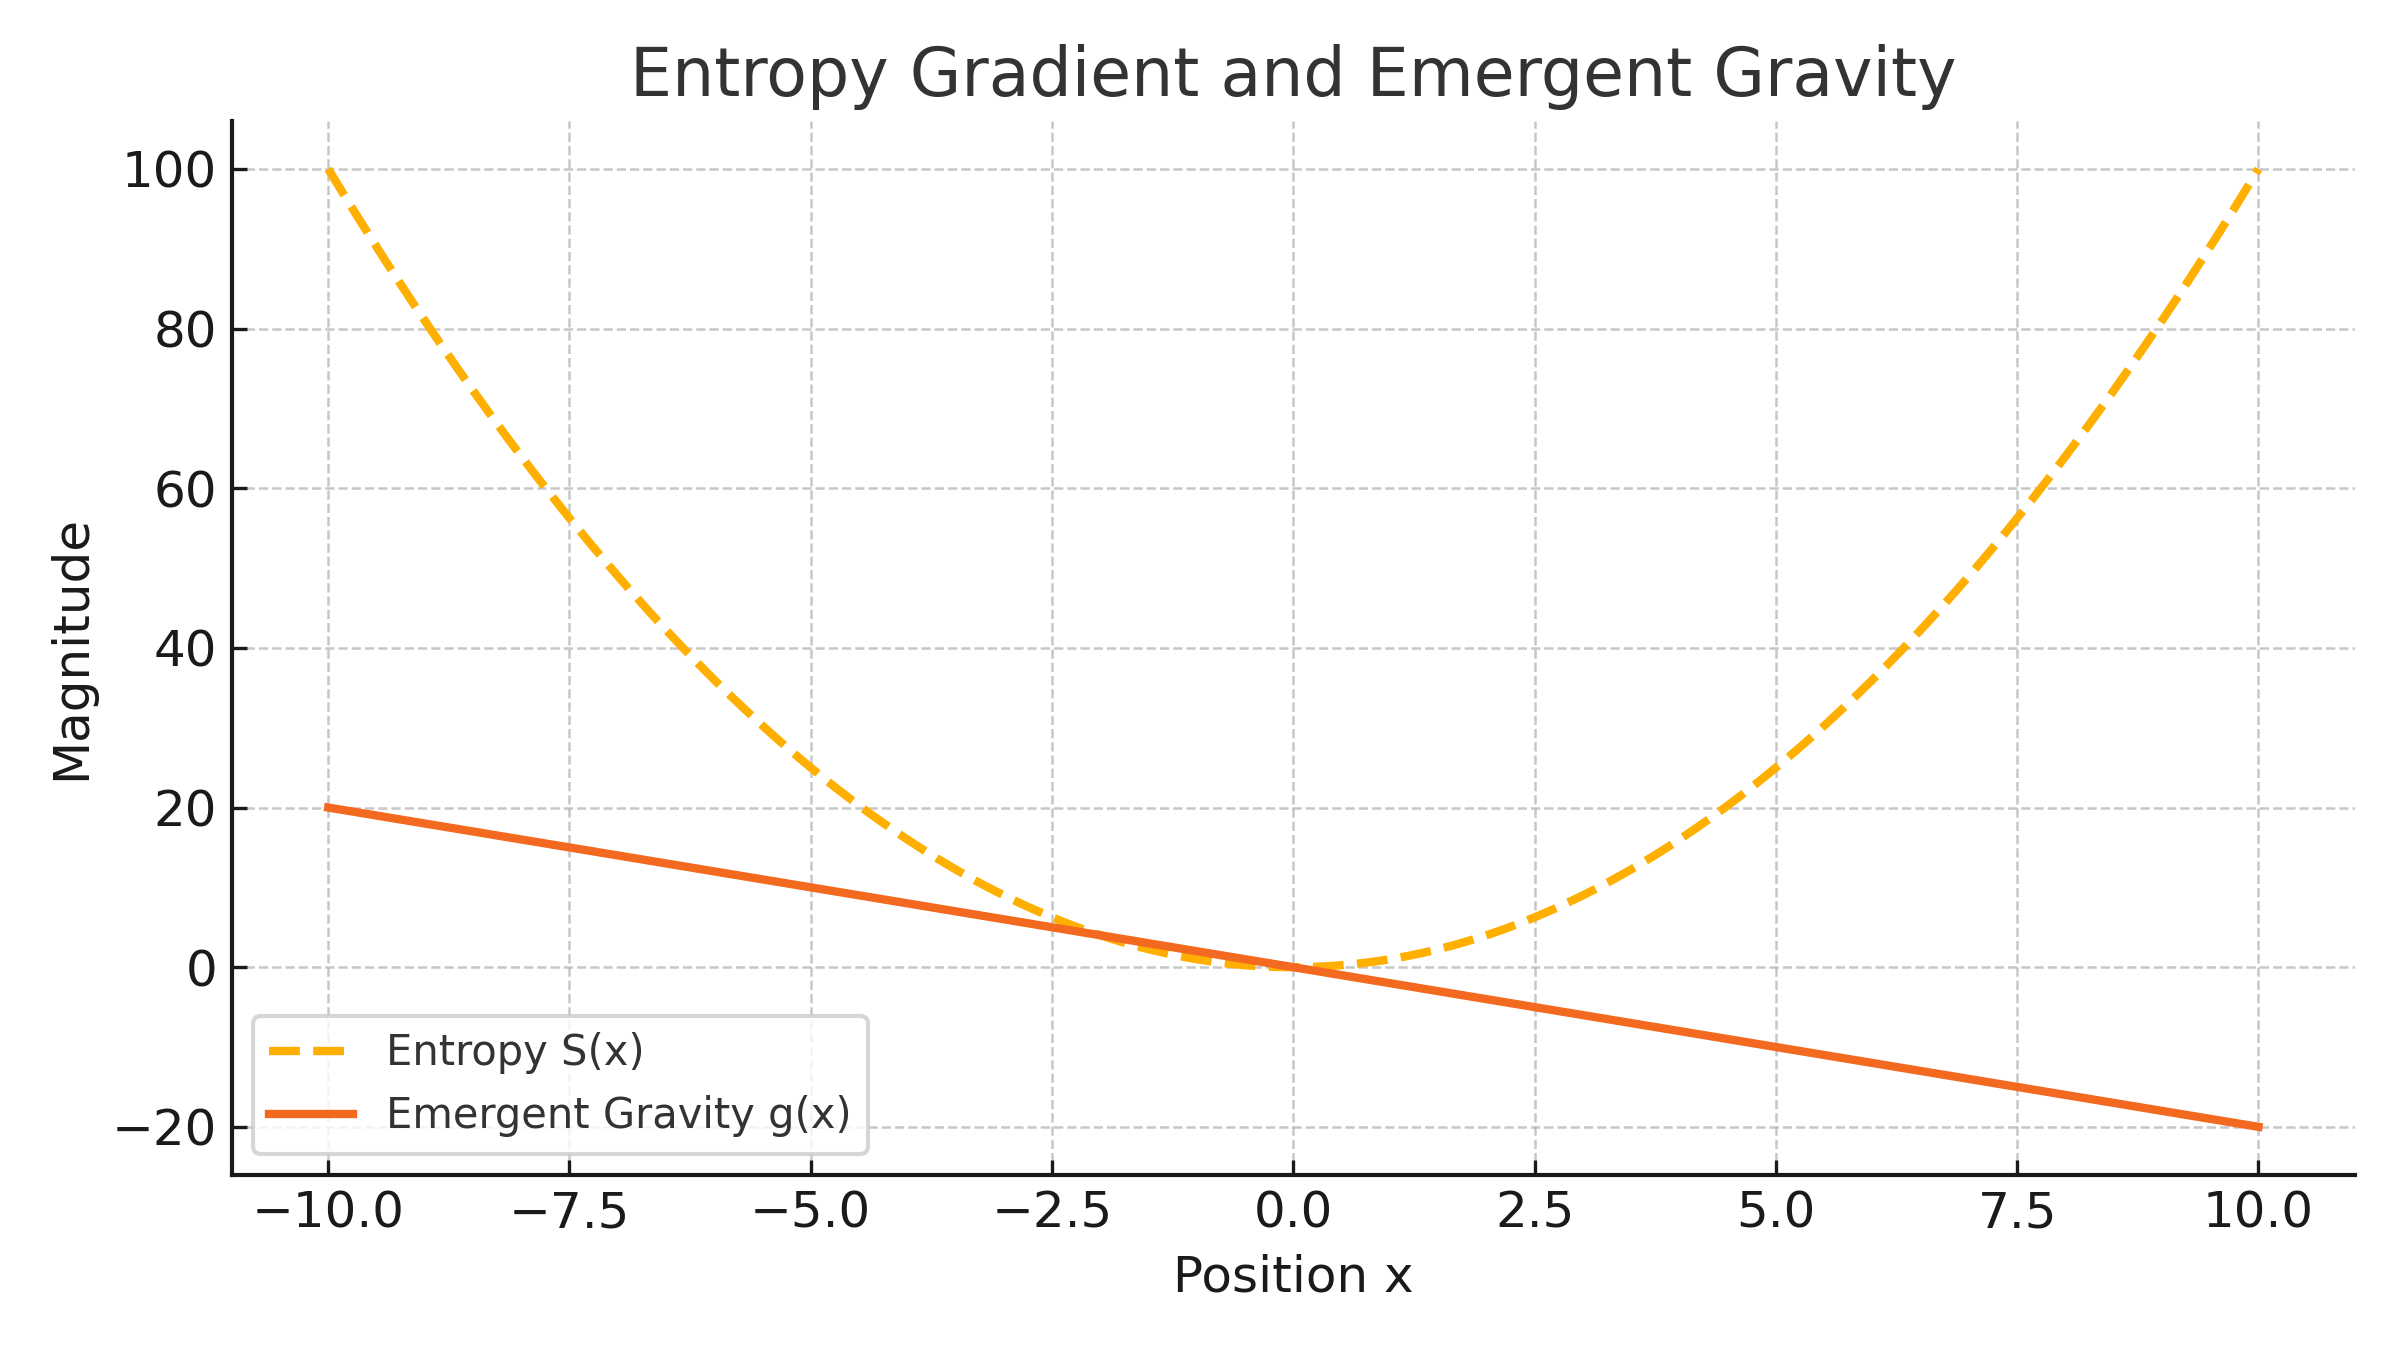
\includegraphics[width=0.85\textwidth]{fig_03_gradient_model.png}
\caption{Entropy gradient as a driver of emergent gravity. The field $g(x) = -\nabla S(x)$ demonstrates how entropy variation produces directional effects.}
\label{fig:gradient_model}
\end{figure}

\clearpage
\begin{figure}[H]
\centering
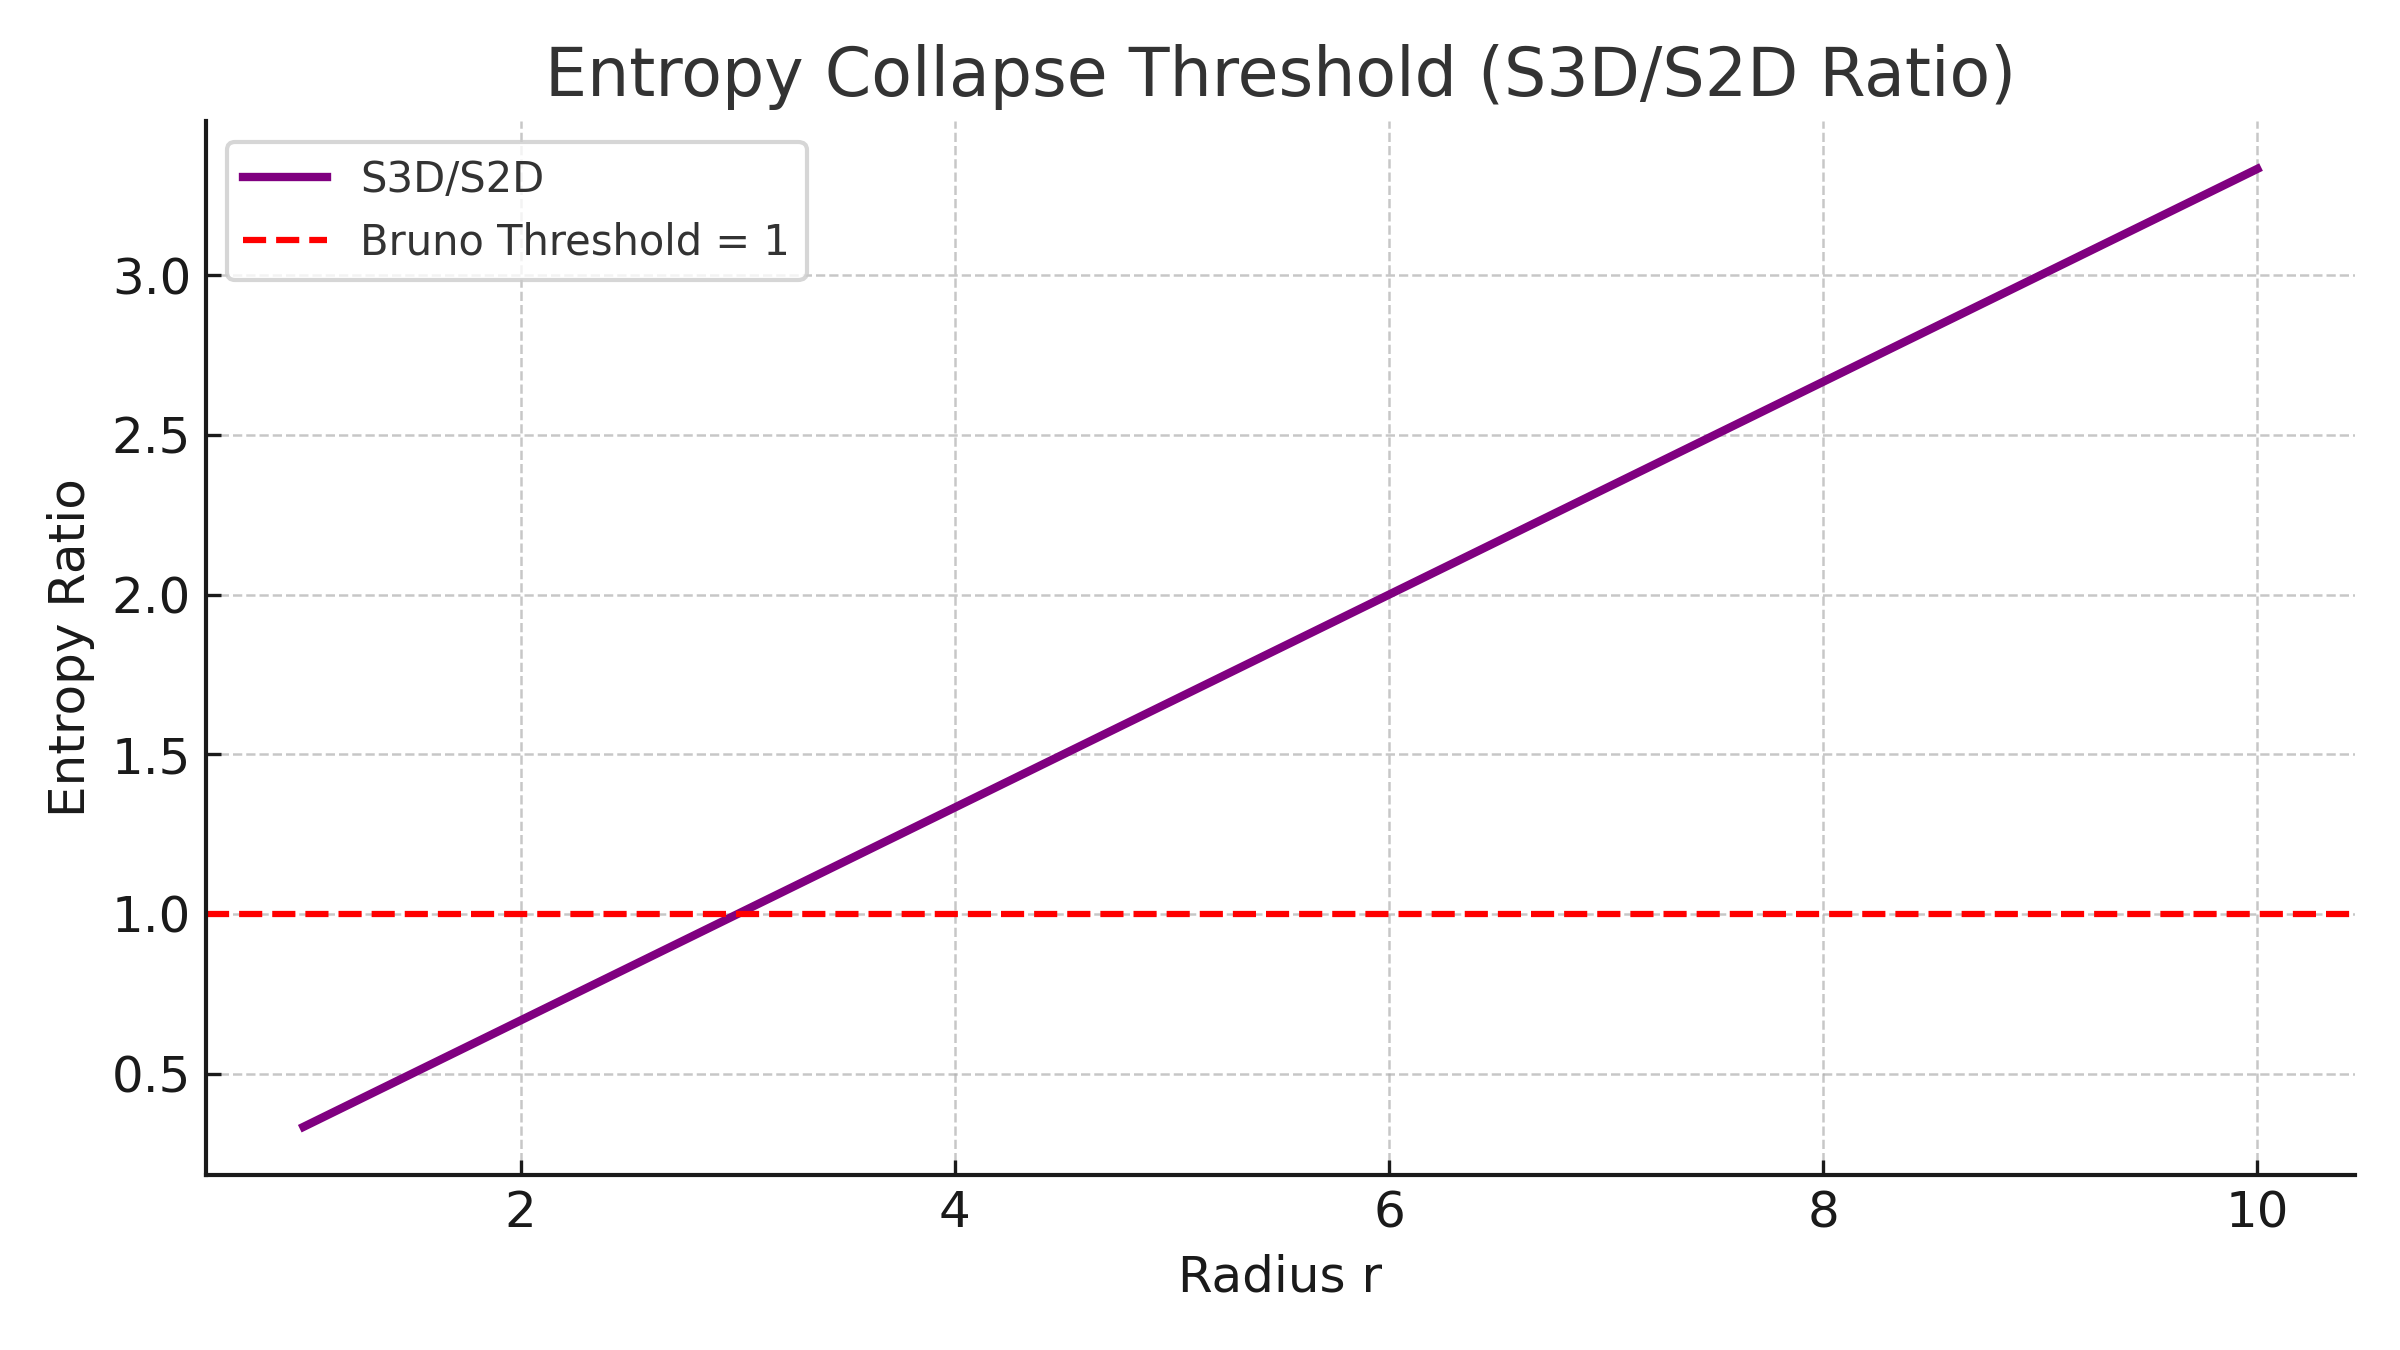
\includegraphics[width=0.85\textwidth]{fig_04_collapse_threshold.png}
\caption{Collapse threshold when the volumetric to surface entropy ratio $S_{3D}/S_{2D}$ reaches the Bruno Constant.}
\label{fig:collapse_threshold_alt}
\end{figure}

\clearpage
\begin{figure}[H]
\centering
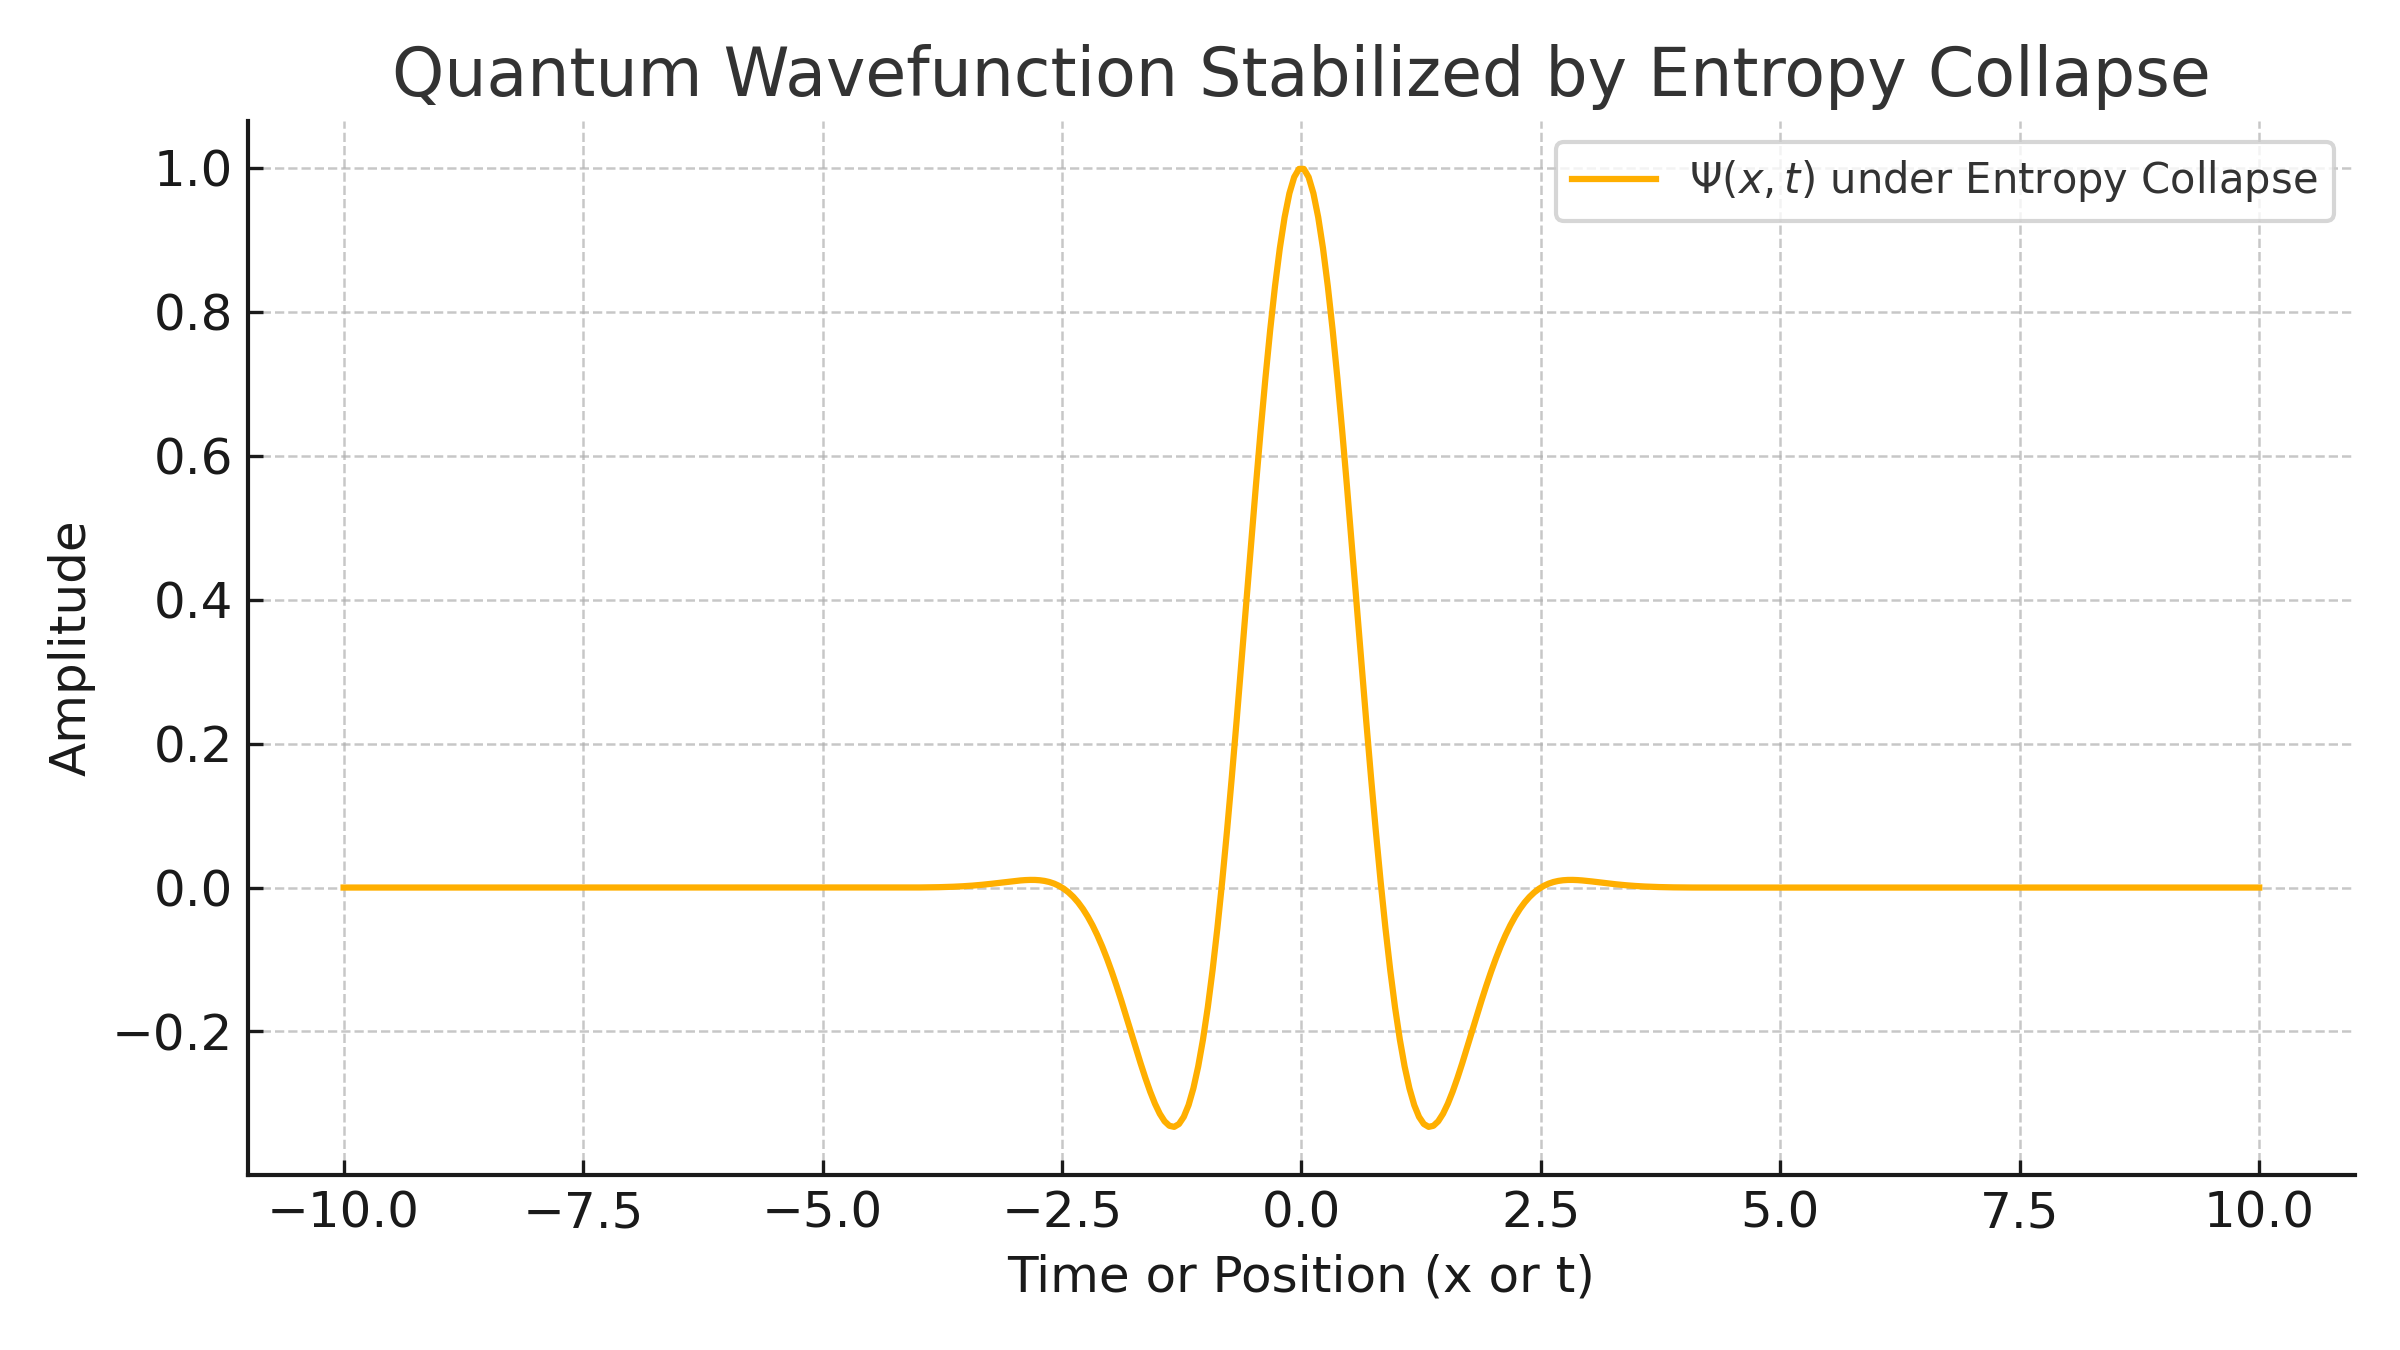
\includegraphics[width=0.85\textwidth]{fig_05_wavefunction_stability.png}
\caption{Wavefunction collapse stabilized by entropy. The envelope reflects entropy flattening near the collapse point.}
\label{fig:wavefunction_stability_exp}
\end{figure}

\clearpage
\begin{figure}[H]
\centering
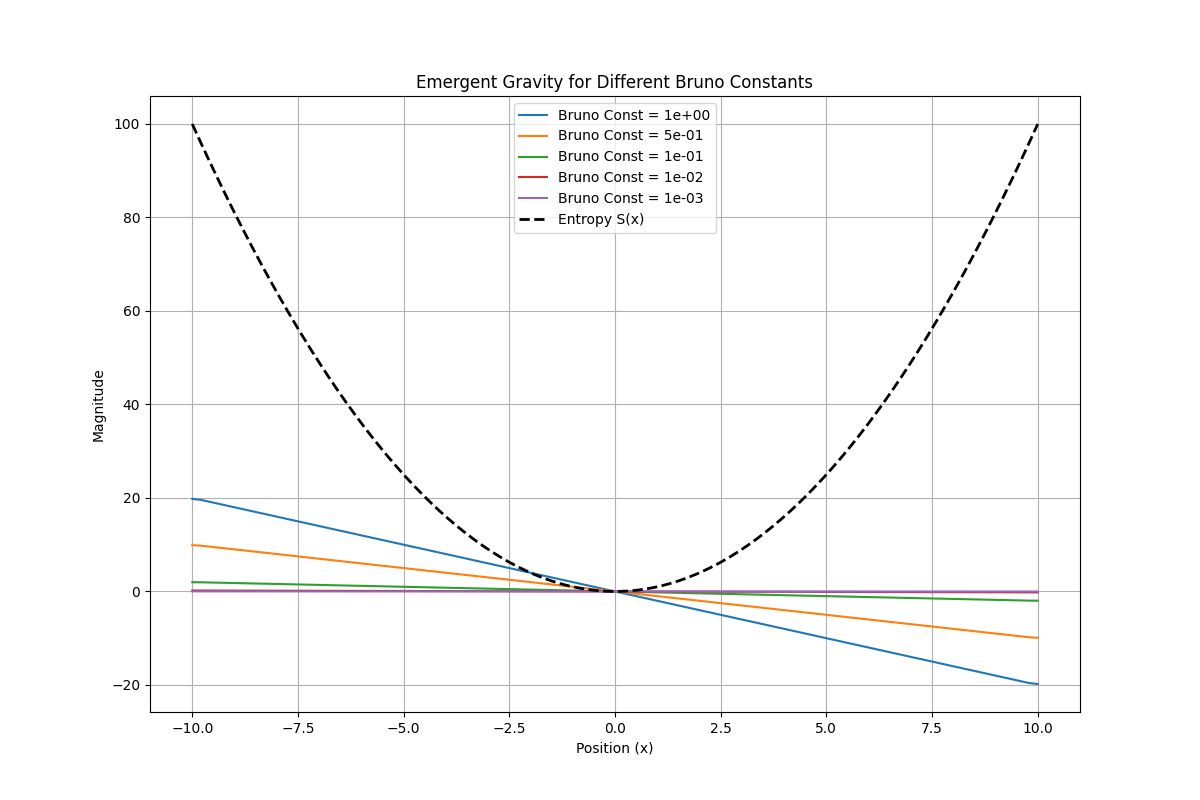
\includegraphics[width=0.85\textwidth]{fig_06_toy_model_entropy.png}
\caption{Toy model showing entropy distribution $S(x)$ and emergent gravity $g(x) = -dS/dx$ across a 1D domain.}
\label{fig:toy_model_final}
\end{figure}

\clearpage
\begin{figure}[H]
\centering
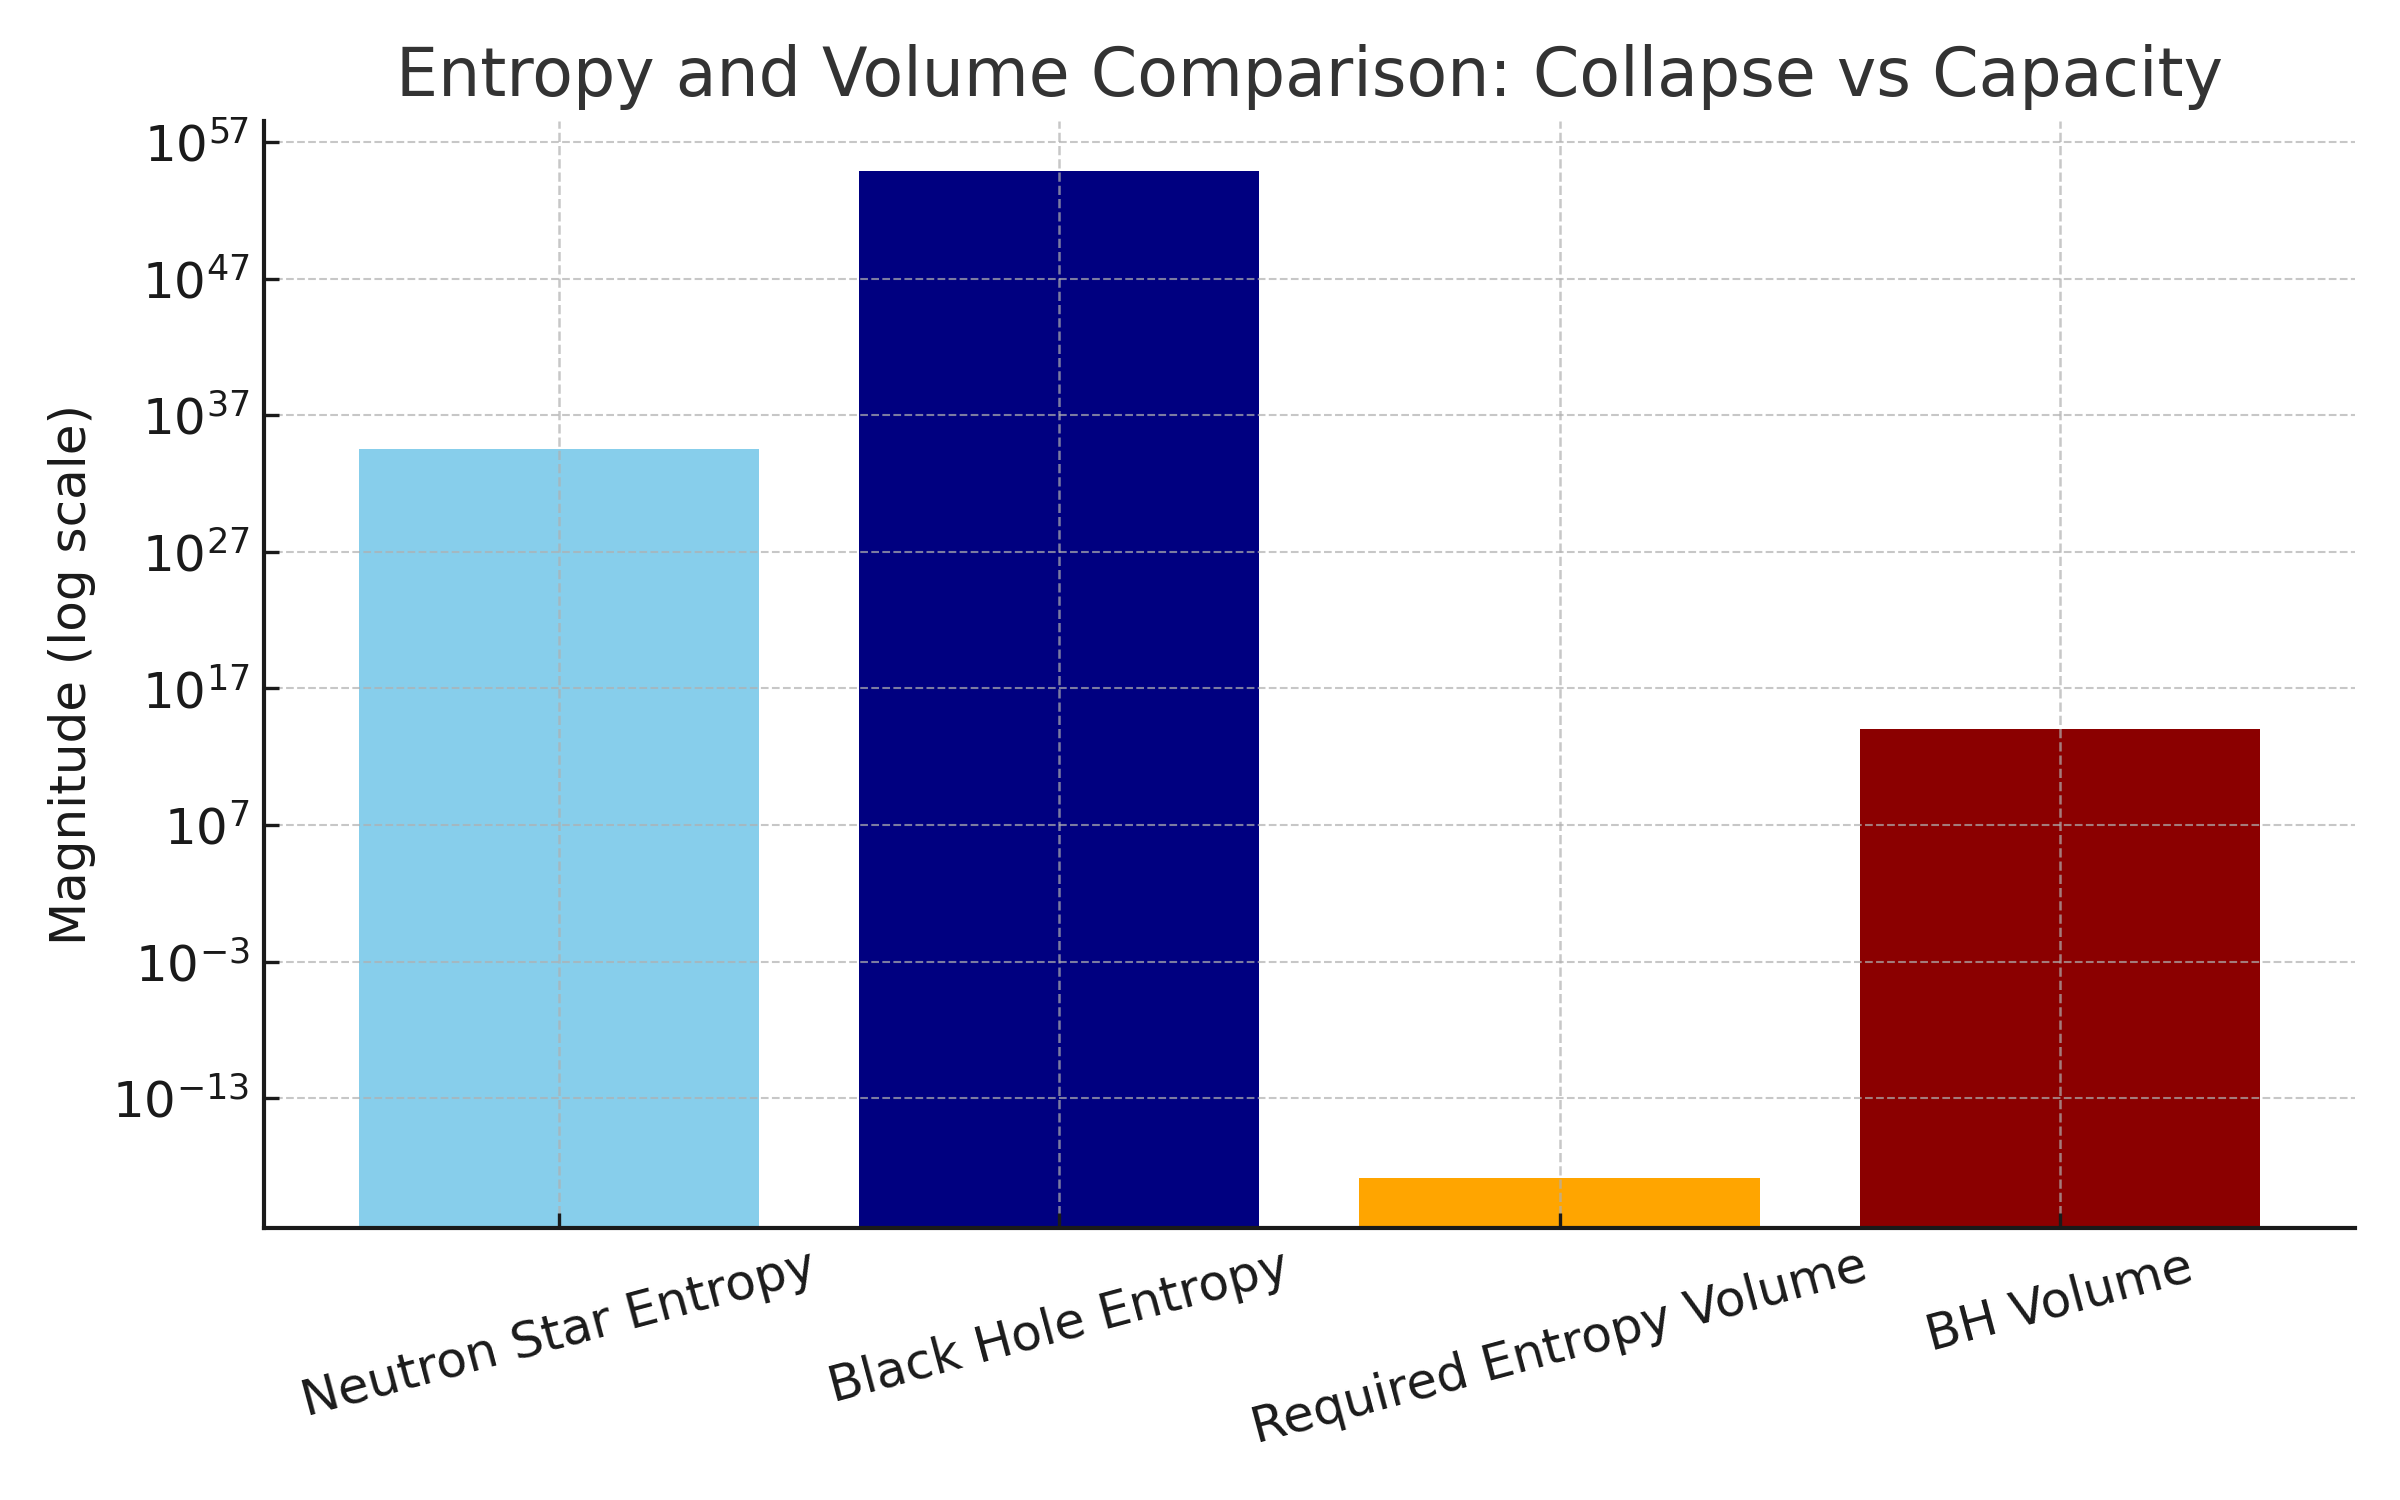
\includegraphics[width=0.85\textwidth]{fig_07_surface_vs_volume.png}
\caption{Entropy and volume mismatch: the required volume to store black hole entropy far exceeds actual Schwarzschild volume, implying the necessity of 2D encoding.}
\label{fig:surface_vs_volume}
\end{figure}

\clearpage
\begin{figure}[H]
\centering
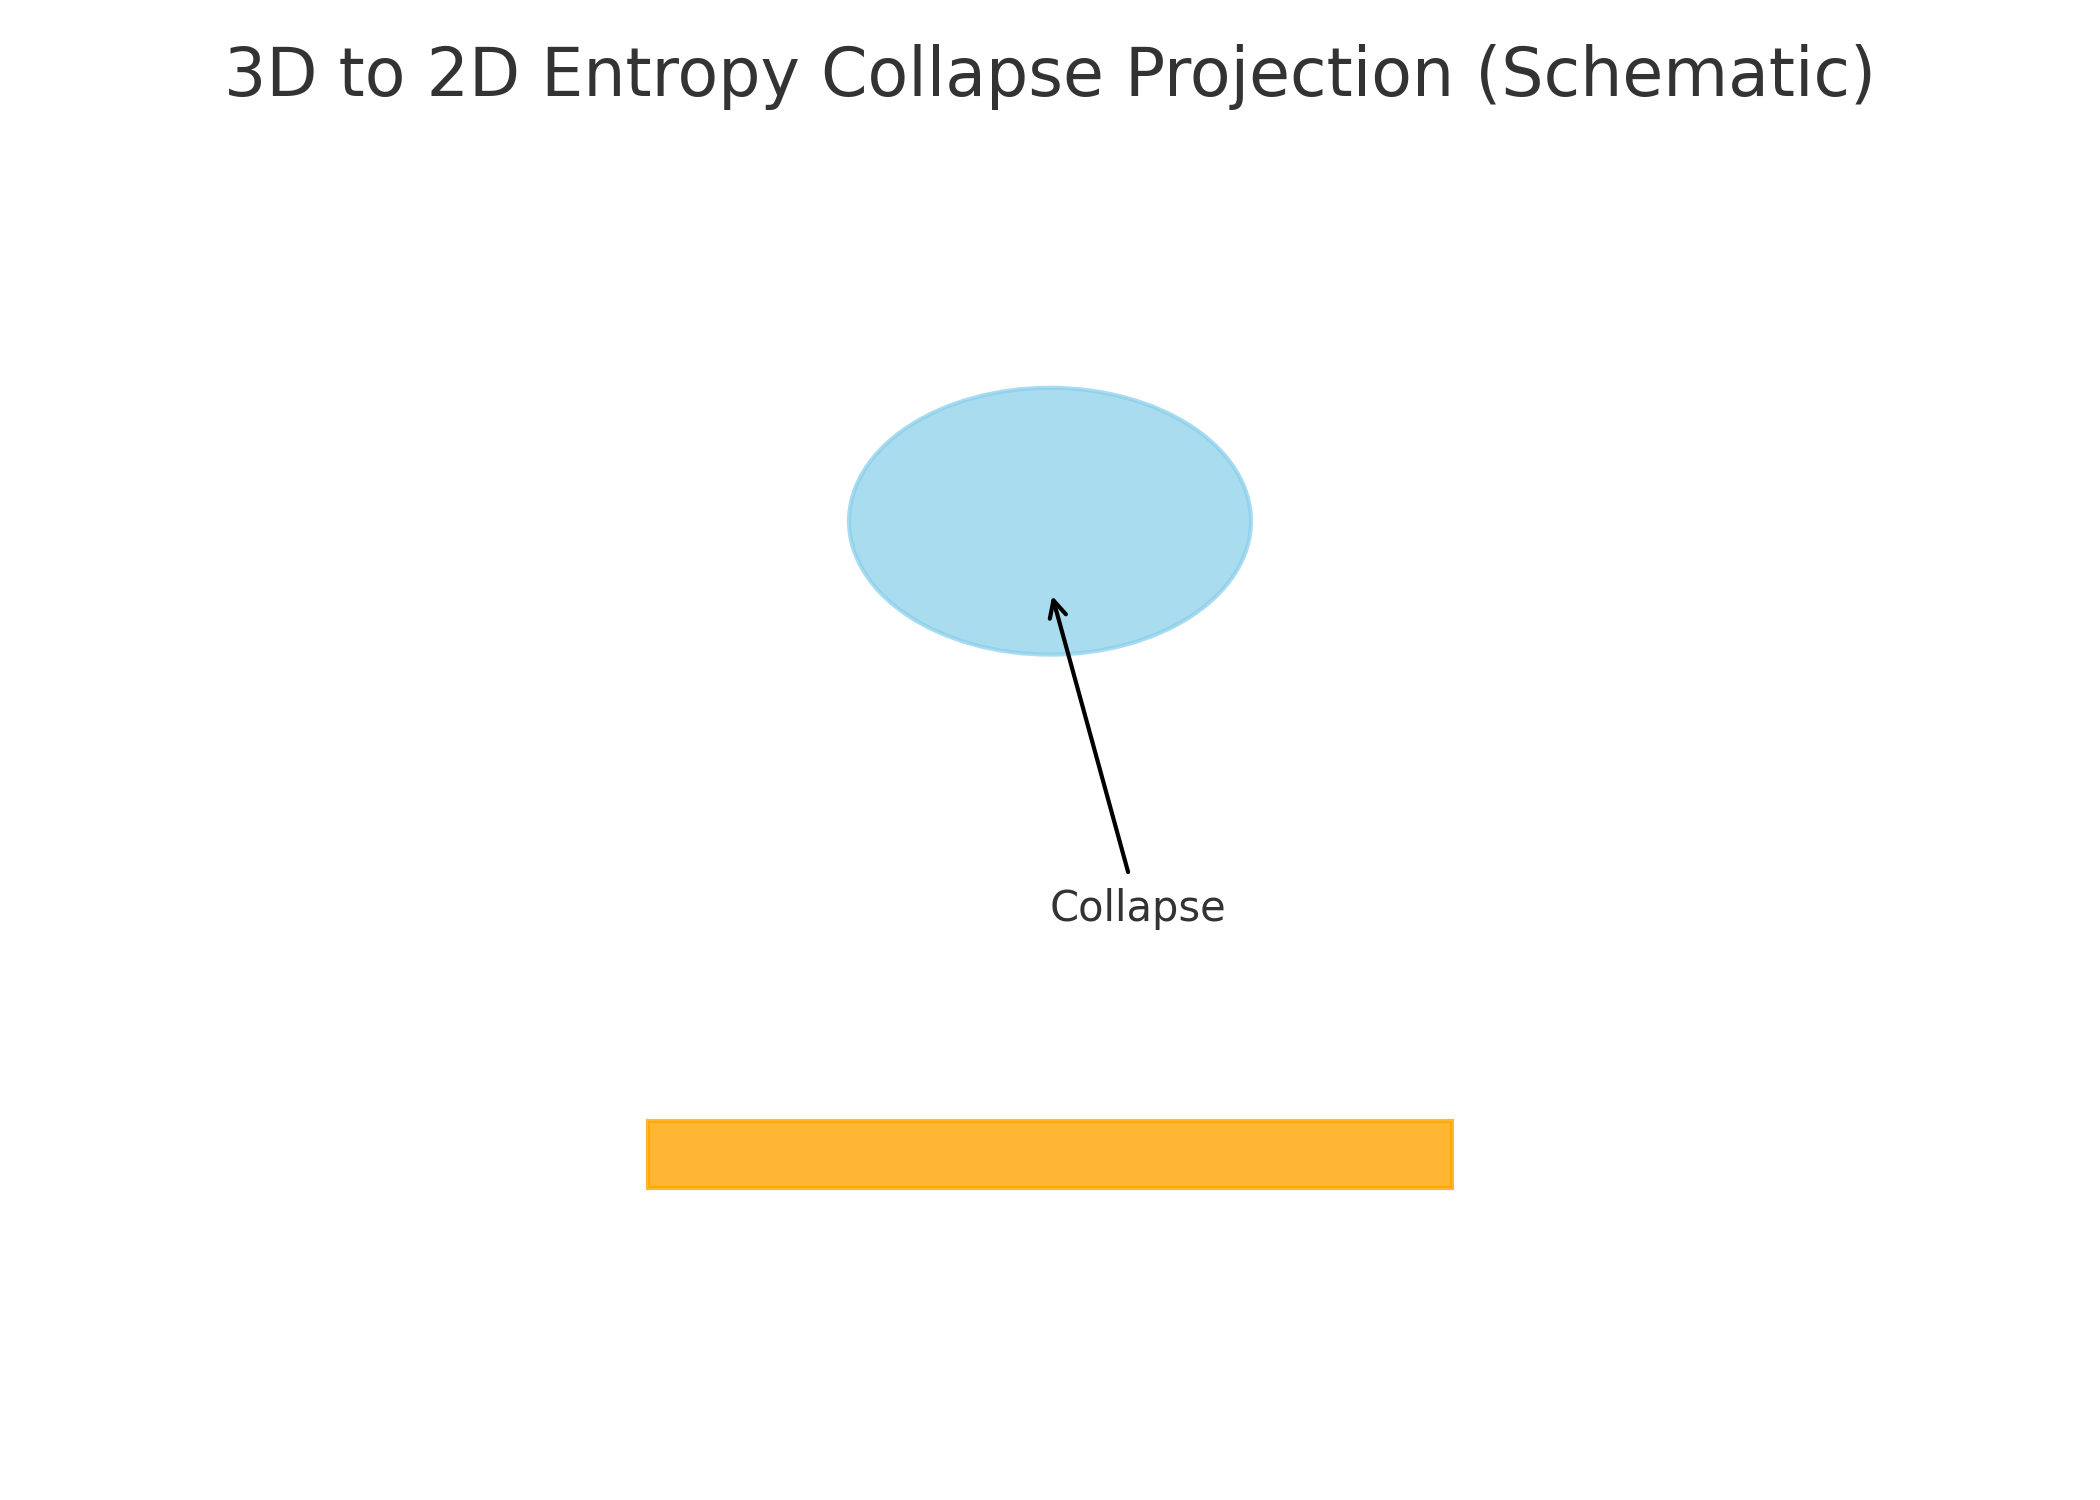
\includegraphics[width=0.85\textwidth]{fig_08_final_projection.png}
\caption{Schematic of entropy collapse: 3D volumetric entropy condensing into a 2D holographic surface.}
\label{fig:final_projection_closeup}
\end{figure}